\section{Improvements of Clustering Algorithm}
\label{sec:clustering_opt}
% 具体来说，我们迭代式地使用MeanShift算法，并预设一个聚类半径R，以及一个类簇的最小样本数量K。在每次迭代中，对于完成聚类的样本，我们检验每个样本到类簇中心的距离是否大于R，并把大于R的样本重新标记为没有聚类。同时，对于样本数量小于K的聚类，我们也把这些类的样本标记为没有聚类。在每次迭代结束，我们把MeanShift的离群点与我们标记出没有聚类的样本重新纳入下一轮地聚类中，直到所有样本类别不再发生变化。我们把我们把伪代码展示在\cref{improved_shift}。
\subsection{Improved MeanShift Algorithm}
\label{sec:improved}
We iteratively apply the MeanShift algorithm with an \camera{adaptive} cluster radius $R$ and a minimum cluster size $K$. 
In each iteration, for the clustered samples, we examine whether the distance between each sample and its cluster center exceeds R, and relabel those samples that exceed this threshold as unclustered. 
For clusters containing fewer than K samples, we mark all samples in these clusters as unclustered. 
At the end of each iteration, we incorporate both the outliers from MeanShift and our marked unclustered samples into the next round of clustering, continuing this process until no further changes occur in sample labels. We present the pseudocode in \cref{algo:improved_meanshift}.

\begin{algorithm}
\caption{Iterative MeanShift Clustering Algorithm}
\label{algo:improved_meanshift}
\begin{algorithmic}[1]
\State \camera{Calculate adaptive radius: $R=\min(\mathrm{estimate\_bandwidth}(Q),U)$}
\State Initialize all labels in the evaluation set to $-1$
\Repeat
    \State Perform MeanShift clustering with radius $R$ on all samples labeled $-1$
    \State Assign new labels to clustered samples
    \For{each newly labeled sample $i$}
        \State Calculate distance $\mathrm{dist}_i$ to its cluster center
        \If{$\mathrm{dist}_i > R$}
            \State Reset label to $-1$
        \EndIf
    \EndFor
    \For{each cluster}
        \If{number of samples in cluster $< K$}
            \State Reset all samples in this cluster to $-1$
        \EndIf
    \EndFor
    \State Renumber all non-$\{-1\}$ newly labeled samples to avoid overlap with old labels
\Until{no label changes}
\end{algorithmic}
\end{algorithm}

In the experiment, $K$ is empirically set to $10$, which has been verified through extensive experiments to be a reasonable and robust value. \camera{To determine the clustering radius $R$, we employ the \textit{estimate\_bandwidth} function from the \textit{sklearn.cluster} library. This utility automatically computes a bandwidth value that balances clustering granularity and stability based on the underlying distribution of the data. The function is governed by a quantile hyperparameter $Q$, which typically ranges from $0.1$ to $0.5$. Given our framework's stringent requirements for minimizing intra-cluster variance, we adopt a conservative value of $Q=0.1$ in practice. Furthermore, considering that sample sizes and difficulty distributions vary significantly across different evaluation sets, the automatically estimated bandwidth may occasionally become excessively large. To mitigate this risk, we introduce a global upper bound $U$ on the bandwidth. Specifically, we define $U = max\_distance/10$, where $\text{max\_distance}$ represents the theoretical maximum distance between any two vectors in the difficulty feature space and $10$ is a empirical constant. In our experimental setup, the feature vectors are 9-dimensional with each element inherently bounded within the range $[0, 1]$. Consequently, the maximum possible Euclidean distance is calculated as $\sqrt{1^2 \times 9} = 3$, yielding an upper bound of $U = 0.3$.}

% The fixed radius $R$ depends only on the value range and dimensionality (i.e., the number of predictive models) of the difficulty feature vectors. In our experiments, we fixed $R=0.3$ for all evaluation sets to ensure consistent overall clustering performance. 

% For experiments with different numbers of small models used for fitting, the value of $R$ needs to be adaptively adjusted due to changes in the dimensionality of the feature vector. For instance, in the experiment of predicting the 12B-parameter model, $R$ was empirically reduced from $0.3$ to $0.2$ to ensure that the intra-class error is reasonable.


\paragraph{Filtering zero-performance samples.}
In the evaluation set, there may exist a few extremely difficult problems that require sufficient model parameters to emerge. All small models may fail to solve these problems even after 100 evaluation attempts, resulting in difficulty feature vectors of all zeros. We refer to these as zero-performance samples. Their presence leads to two issues:
\begin{enumerate}[leftmargin=1.5em]
    \item Zero performance on small models does not necessarily indicate zero accuracy on large models. For these samples, we cannot estimate when emergence will occur or predict large model metrics.
    \item During clustering, they may be confused with other low-performing but non-zero samples. Including them in the same cluster would lower the expected accuracy of that cluster, leading to inaccurate fitting and extrapolation later.
\end{enumerate}

Therefore, we pre-filter these zero-performance samples before clustering, treating them as outliers that do not participate in the clustering process. 
% This approach eliminates the need to consider their metrics under large models during subsequent extrapolation and prevents disruption to the clustering of the remaining samples.
This approach obviates the necessity of considering their metrics under large models during subsequent extrapolation, and prevents disruption to the clustering of the remaining samples.



\subsection{Smoothing Techniques}
\label{sec:smoothing}
% \noindent\textbf{Horizontal smoothing: adjacent checkpoint smoothing.}
Metric fluctuations of individual samples in downstream tasks are not solely due to limited sampling. Another potential factor is noise from uneven data distribution in recent training batches. Therefore, in addition to performing 100 evaluations to mitigate sampling variance, we evaluated 100 times on each of the adjacent checkpoints before and after the selected model. We then averaged these accuracy expectation values across three checkpoints, further reducing sampling variance while offsetting noise from uneven training data distribution. This approach also reduces the number of zero-performance samples, further improving clustering and prediction effectiveness.






\section{Proof of Theorem 1}
\label{sec:prop_proof}
We use \cref{proof:am_gm} to derive the scaling law for downstream task performance (\cref{main:proof:task_scaling_law}).
\begin{lemma}[Arithmetic-geometric mean difference]
\label{proof:am_gm}
For any sequence of positive real numbers $\{x_i\}_{i=1}^n$, let:
\begin{itemize}
    \item $\mu_a = \frac{1}{n}\sum_{i=1}^n x_i$ be the arithmetic mean;
    \item $\mu_g = \prod_{i=1}^n x_i^{1/n}$ be the geometric mean; 
    \item $\sigma^2 = \frac{1}{n}\sum_{i=1}^n (x_i-\mu)^2$ be the variance.
\end{itemize}
Then the difference between the arithmetic mean and geometric mean can be estimated as:
\begin{align}
    \Delta &= \mu_a-\mu_g = \frac{1}{n}\sum_{i=1}^n x_i-\left(\prod_{i=1}^n x_i\right)^{\frac{1}{n}} =\frac{\sigma^2}{2\mu_a}+o(\sigma^2).
\end{align}
\end{lemma}
\begin{proof}
Taking the logarithm of the geometric mean $\mu_g$:
\begin{align}
    \log (\mu_g)=\frac{1}{n} \sum_{i=1}^n \log x_i.
\end{align}

Using Taylor expansion of $\log x$ around $\mu$:
\begin{align}
    \log x = \log \mu + \frac{x-\mu}{\mu}-\frac{(x-\mu)^2}{2\mu^2}+o\left((x-\mu)^2\right)
\end{align}
We can simplify:
\begin{align*}
 \frac{1}{n} \sum_{i=1}^n \log x_i
=& \log \mu + \frac{1}{n}\sum_{i=1}^n\left(\frac{(x_i-\mu_a)}{\mu_a}-\frac{(x_i-\mu_a)^2}{2\mu_a^2}+o\left((x_i-\mu_a)^2\right)\right) \\
=& \log\mu +\frac{1}{\mu} \underbrace{\left(\frac{1}{n}\sum_{i=1}^nx_i -\mu_a\right)}_{\text{equal to 0}} + \frac{1}{2\mu_a^2}\underbrace{\left(\frac{1}{n}\sum_{i=1}^n(x_i-\mu_a)^2\right)}_{\sigma^2}+o\left(\frac{1}{n}\sum_{i=1}^n(x_i-\mu_a)^2\right)\\
=& \log \mu -\frac{\sigma^2}{2\mu^2} + o(\sigma^2).
\end{align*}
Therefore:
\begin{align}
    \mu_a-\mu_g = \mu_a \left(1-\exp{\left(-\frac{\sigma^2} {2\mu^2}\right)}\right) + o(\sigma^2).
\end{align}
When $\frac{\sigma^2}{2\mu^2}$ is small, this can be approximated as:
\begin{align}
    \Delta \approx \frac{\sigma^2}{2\mu_a}.
\end{align}
\end{proof}

\begin{theorem}[Scaling Law for Downstream Task Performance]
\label{supp:proof:task_scaling_law}
Consider a language model $M_C$ trained with compute budget $C$ and a set of downstream tasks $\mathcal{P}$. Under the following assumptions:
Assumption 1 (Power-law scaling of answer loss): the expected answer loss follows:
\begin{equation}
L_{\mathcal{P}}(C) := \mathbb{E}_{(q,a_{\text{true}}) \sim \mathcal{P}}[L(q, a_{\text{true}}; C)] = \alpha C^{-\beta} + \gamma,
\end{equation}
where $\alpha, \beta, \gamma > 0$ are task-specific constants, with $\gamma$ representing the irreducible loss.

Assumption 2 (Unique deterministic answers): Each question has a unique deterministic answer. The model receives score $1$ if and only if $M_C$ outputs $a_{\text{true}}$, and $0$ otherwise.

Assumption 3 (Accuracy decomposition): The expected accuracy decomposes as:
\begin{equation}
\mathbb{E}_{T \sim \mathcal{P}}[\mathrm{Acc}(C)] = g + (1-g) \cdot \mathbb{E}_{(q,a_{\text{true}}) \sim \mathcal{P}}[p(a_{\text{true}}|q, M_C)],
\end{equation}
where $g \in [0,1]$ is the random guessing baseline.

Then, the expected accuracy on task set $\mathcal{P}$ can be modeled as:
\begin{equation}
\mathbb{E}_{\mathcal{P}}[\mathrm{Acc}(C)] = g+(1-g)\left(\exp{(-\alpha C^{-\beta}-\gamma)} + \frac{\sigma_L^2(C)}{2\mu_L(C)} \right)+ o\left(\sigma_L^2(C)\right),
\end{equation}
where $\mu_L(C) = \mathbb{E}_{(q,a_{\text{true}}) \sim \mathcal{P}}[L(q, a_{\text{true}}; C)]$ is the mean loss and $\sigma_L^2(C) = \mathrm{Var}_{(q,a_{\text{true}}) \sim \mathcal{P}}[L(q, a_{\text{true}}; C)]$ is the loss variance across the task set.
\end{theorem}

\begin{proof}
For a task $T=(q,a_{\text{true}}) \in \mathcal{P}$, under assumption 2, $a_{\text{true}}$ is deterministic and unique, thus $p(a_{\text{true}}|q, M_C)$ can be decomposed into token-wise auto-regressive loss.
\begin{align}
\label{eq:loss_passrate}
    -\log (p(a_{\text{true}}|q, M_C))&= -\log\left(\prod_{i=1}^k p(t_i|q,t_{<i};M_C)\right) \\ 
    &=-\sum_{i=1}^k\log\left(p(t_i|q,t_{<i};M_C)\right)\\ 
    &=L(q,a_{\text{true}};C).
\end{align}
Then take the exponential of both sides, and then take the expectation with respect to different tasks in the evaluation set $p=(q,\mathrm{ans})\in P$. We note that both $p_{\mathrm{ans}}$ and $\mathrm{loss}_{\mathrm{ans}}$ are functions of $C$.
\begin{align}
\mathbb{E}_p[p(a_{\text{true}}|q, M_C)]&=\mathbb{E}_p[\exp(-L(q,a_{\text{true}};C)] =\frac{1}{n}\sum_{(q, a_{\text{true}})\in P} \exp(-L(q,a_{\text{true}};C)).
\end{align}
We can adopt \cref{proof:am_gm} to switch from arithmetic mean to geometric mean of $\mathrm{loss}$, and apply the power law assumption 1. 
\begin{align}
\label{eq:loss_function}
    \frac{1}{n}\sum_{(q, a_{\text{true}})\in P} \exp(-L(q,a_{\text{true}};C)) =& \exp{\underbrace{\left(-\frac{1}{n}\sum_{(q, a_{\text{true}})\in P}L(q,a_{\text{true}};C)\right)}_{\text{use loss scaling law}}} + \frac{\sigma_L^2(C)}{2\mu_L(C)} + o\left(\sigma_L^2(C)\right) \\
    =& \exp{(-\alpha C^{-\beta}-\gamma)} + \frac{\sigma_L^2(C)}{2\mu_L(C)} + o\left(\sigma_L^2(C)\right),
\end{align}
where $n$ in the number of tasks in $\mathcal{P}$, and $\mu$, $\sigma^2$ follow definitions in the proposition.

Finally, we use assumption 3 to align the answer passrate and the accuracy metric. 
\begin{align}
\mathbb{E}_{T \sim \mathcal{P}}[\mathrm{Acc}(C)] &= g + (1-g) \cdot \mathbb{E}_{(q,a_{\text{true}}) \sim \mathcal{P}}[p(a_{\text{true}}|q, M_C)] \\
&=g+\frac{(1-g)}{n}\sum_{(q, a_{\text{true}})\in P} \exp(-L(q,a_{\text{true}};C)) \\
&=g+(1-g)\left(\exp{(-\alpha C^{-\beta}-\gamma)} + \frac{\sigma_L^2(C)}{2\mu_L(C)} \right)+ o\left(\sigma_L^2(C)\right) 
\end{align}


\end{proof}

\paragraph{Rationality of Assumption 3}
Assumption 3 is designed to accommodate tasks with finite answer sets. For such tasks, when calculating $\text{Acc}(C)$, possibilities outside the answer set are disregarded. When $p(a_{\text{true}} \mid q, M_C)$ approaches 0, $\text{Acc}(C)$ is at the level of a random guess, $g$. When $p(a_{\text{true}} \mid q, M_C)$ approaches 1, $\text{Acc}(C)$ is close to $p(a_{\text{true}} \mid q, M_C)$. This assumption implies a linear relationship between $\text{Acc}(C)$ and the probability in the $(0,1)$ interval. The theorem itself is also effective for tasks with open answer sets, where the probability of a correct random guess can be assumed to be 0 (i.e., $g=0$).



% \renewcommand{\thefigure}{C\arabic{figure}}
% \renewcommand{\thetable}{C\arabic{table}}
% \renewcommand{\theproposition}{C.\arabic{proposition}}
% \setcounter{table}{0} 
% \setcounter{figure}{0} 
% \camera{
% \section{Relation Between Fitting RMSE and Prediction Error }

% \subsection{Model Setup}

% Let $\theta = (a,b,c)^\top \in \Theta \subset \mathbb{R}^3$.
% Define the deterministic mean function
% \begin{equation}
% \mu(x;\theta)
% := \exp\!\big(-a x^{-b} - c\big).
% \end{equation}

% \paragraph{Data Generating Process (DGP).}
% We observe i.i.d.\ pairs $(x_i,y_i)_{i=1}^N$ satisfying
% \begin{equation}
% y_i = \mu(x_i;\theta^\ast)\exp(-\epsilon_i),
% \end{equation}
% where $\theta^\ast$ is the true parameter and
% \[
% \mathbb{E}[\epsilon_i]=0,
% \qquad
% \mathrm{Var}(\epsilon_i)=\sigma^2,
% \qquad
% \sigma^2 \text{ is small}.
% \]

% Let $\hat\theta$ be a consistent estimator of $\theta^\ast$ (e.g.\ nonlinear least squares),
% and define the fitted values
% \[
% \hat y_i := \mu(x_i;\hat\theta).
% \]

% \paragraph{In-sample RMSE (original $y$-space).}
% \begin{equation}
% \mathrm{RMSE}_y^2
% :=
% \frac{1}{N}\sum_{i=1}^N (y_i-\hat y_i)^2.
% \end{equation}

% \paragraph{Out-of-sample MSPE.}
% For a fixed extrapolation point $x_0$, define
% \[
% y_0 = \mu(x_0;\theta^\ast)\exp(-\epsilon_0),
% \qquad
% \hat y_0 = \mu(x_0;\hat\theta),
% \]
% and
% \[
% \mathrm{MSPE}_y(x_0)
% =
% \mathbb{E}\big[(y_0-\hat y_0)^2\big].
% \]

% \subsection{Proposition}

% \begin{proposition}
% Assume:

% \begin{enumerate}
% \item $\hat\theta$ is consistent and asymptotically normal:
% \[
% \sqrt{N}(\hat\theta-\theta^\ast)
% \Rightarrow
% \mathcal{N}(0,\Sigma_\theta).
% \]
% \item $\sigma^2$ is sufficiently small so that first-order Delta expansions are valid.
% \end{enumerate}

% Then for any fixed $x_0$,
% \begin{equation}
% \mathrm{MSPE}_y(x_0)
% \approx
% \mathrm{RMSE}_y^2
% \cdot
% \frac{\hat y_0^2}{\frac{1}{N}\sum_{i=1}^N \hat y_i^2}
% \cdot
% \left(
% 1
% +
% \nabla_\theta \log \mu(x_0;\hat\theta)^\top
% \widehat{\Sigma}_\theta
% \nabla_\theta \log \mu(x_0;\hat\theta)
% \right).
% \end{equation}

% The first ratio is the heteroskedastic scaling factor.
% The second term is the parameter uncertainty inflation factor.
% \end{proposition}

% \subsection{Proof}

% \begin{proof}

% \noindent\textbf{Step 1: Heteroskedastic variance in $y$-space.}

% Since
% \[
% y_i = \mu(x_i;\theta^\ast)\exp(-\epsilon_i),
% \]
% apply a first-order Delta expansion:
% \[
% \exp(-\epsilon_i) \approx 1-\epsilon_i.
% \]
% Thus
% \[
% y_i \approx \mu(x_i;\theta^\ast)(1-\epsilon_i),
% \]
% and the $y$-space residual is
% \[
% e_{y,i}
% =
% y_i-\mu(x_i;\theta^\ast)
% \approx
% -\mu(x_i;\theta^\ast)\epsilon_i.
% \]

% Therefore,
% \begin{equation}
% \mathrm{Var}(y_i\mid x_i)
% \approx
% \mu(x_i;\theta^\ast)^2\sigma^2.
% \end{equation}

% This proves the multiplicative heteroskedastic structure.

% \noindent\textbf{Step 2: Linking RMSE to $\sigma^2$.}

% For large $N$, the estimation error term is $o_p(1)$, hence
% \[
% \mathrm{RMSE}_y^2
% \approx
% \frac{1}{N}
% \sum_{i=1}^N
% \mu(x_i;\theta^\ast)^2
% \sigma^2.
% \]

% Using plug-in consistency $\mu(x_i;\theta^\ast)\approx\hat y_i$ gives

% \begin{equation}
% \sigma^2
% \approx
% \frac{\mathrm{RMSE}_y^2}
% {\frac{1}{N}\sum_{i=1}^N \hat y_i^2}.
% \end{equation}

% \noindent\textbf{Step 3: MSPE decomposition.}

% At $x_0$,
% \[
% y_0-\hat y_0
% \approx
% -\mu(x_0;\theta^\ast)\epsilon_0
% -
% \nabla_\theta \mu(x_0;\theta^\ast)^\top
% (\hat\theta-\theta^\ast).
% \]

% Since the two terms are asymptotically uncorrelated,

% \begin{equation}
% \mathrm{MSPE}_y(x_0)
% \approx
% \mu(x_0;\theta^\ast)^2\sigma^2
% +
% \nabla_\theta \mu(x_0;\theta^\ast)^\top
% \mathrm{Var}(\hat\theta)
% \nabla_\theta \mu(x_0;\theta^\ast).
% \end{equation}

% Factorizing $\mu(x_0;\theta^\ast)^2$ yields

% \begin{equation}
% \mathrm{MSPE}_y(x_0)
% \approx
% \mu(x_0;\theta^\ast)^2\sigma^2
% \left(
% 1
% +
% \nabla_\theta \log \mu(x_0;\theta^\ast)^\top
% \frac{\Sigma_\theta}{N}
% \nabla_\theta \log \mu(x_0;\theta^\ast)
% \right).
% \end{equation}

% Substituting the expression for $\sigma^2$ proves the result.
% \end{proof}

% In our case, fitting small models have much lower score ($\hat{y}_i^2$) than target model($\hat{y}_0^2$), which makes $\mathrm{MSPE} > 
% \mathrm{RMSE}^2$. Clusters with high fitting RMSE usually have poor prediction accuracy.
% }
\section{Additional Ablation Studies}
\label{sec:additional_ablation}

\subsection{\anno{The Criteria for Extrapolatable Subsets}}
\label{sec:criteria}
\labubu{The criteria for fitting the extrapolation formula (\cref{eq:fitting}) are designed to ensure the following:}
\labubu{
\begin{enumerate}[label=\arabic*,leftmargin=1.5em]
    \item $a > 0$ and $b > 0$: These ensure that accuracy is an increasing function of compute. Larger values of a and b signify that task performance scales more distinctly with compute, leading to fitting curves with better scaling properties and differentiability.
    \item $c \geq 0$: This ensures the extrapolated curve's maximum value is less than or equal to $1$. An excessively large c implies that the fitting curve has a very low ceiling, which is characteristic of task subsets with poor scaling properties. These are thus considered non-extrapolatable.
\end{enumerate}
}

\labubu{We conducted an ablation study on these parameters, as shown in \cref{tab:abc}. Starting from our baseline criteria ($a > 1$, $b > 0.1$, $0 \leq c < 1$), we individually relaxed the constraints on a, b, and c, and also observed the effect of removing the thresholds entirely.}


\begin{table*}[!t]
\small
\setlength{\tabcolsep}{1.8pt} % 保留原列间距设置
\centering
\caption{\labubu{Prediction errors (EE$\downarrow$, FE$\downarrow$) across criteria of extrapolatable subsets.}}
\begin{tabular}{c|cc|cc|cc|cc|cc}
\toprule
\multirow{3}{*}{\makecell[c]{Metric /\\Task Set}} & \multicolumn{2}{c|}{\makecell[c]{Baseline\\($a > 1$, $b > 0.1$, $0 \leq c < 1$)}} & \multicolumn{2}{c|}{\makecell[c]{Ablate a\\($a > 0.5$)}} & \multicolumn{2}{c|}{\makecell[c]{Ablate b\\($b > 0.05$)}} & \multicolumn{2}{c|}{\makecell[c]{Ablate c\\($0 \leq c < 0.5$)}} & \multicolumn{2}{c}{\makecell[c]{w/o threshold}} \\
\cmidrule(lr){2-11}
& EE$\downarrow$ & FE$\downarrow$ & EE$\downarrow$ & FE$\downarrow$ & EE$\downarrow$ & FE$\downarrow$ & EE$\downarrow$ & FE$\downarrow$ & EE$\downarrow$ & FE$\downarrow$ \\
\midrule
% 单个任务集行
GSM8k & 0.31 & 2.68 & 0.31 & 2.68 & 0.31 & 2.68 & 0.31 & 2.68 & 4.05 & 4.35 \\
MATH & 0.84 & 0.79 & 0.84 & 0.79 & 0.84 & 0.79 & 1.04 & 0.94 & 0.40 & 0.38 \\
BBH & 0.54 & 0.47 & 0.54 & 0.47 & 0.54 & 0.47 & 0.17 & 2.04 & 5.39 & 5.33 \\
TriviaQA & 1.56 & 1.97 & 1.57 & 1.96 & 1.56 & 1.97 & 1.05 & 1.42 & 2.82 & 3.77 \\
MBPP & 1.61 & 2.42 & 1.61 & 2.42 & 1.61 & 2.42 & 1.61 & 2.42 & 1.55 & 1.73 \\
AGIEval & 1.11 & 1.64 & 1.11 & 1.64 & 1.11 & 1.64 & 0.08 & 1.35 & 2.24 & 2.38 \\
DROP & 1.44 & 1.05 & 0.24 & 1.05 & 0.29 & 0.96 & 1.71 & 3.59 & 2.17 & 1.83 \\
MMLU-pro & 1.26 & 1.39 & 1.26 & 1.39 & 1.26 & 1.39 & 2.88 & 3.27 & 1.00 & 1.10 \\
\midrule
% 整体指标行
Mean & 1.08 & 1.55 & \textbf{0.94} & 1.55 & \textbf{0.94} & \textbf{1.54} & 1.11 & 2.21 & 2.45 & 2.61 \\
Max & \textbf{1.61} & \textbf{2.68} & \textbf{1.61} & \textbf{2.68} & \textbf{1.61} & \textbf{2.68} & 2.88 & 3.59 & 5.39 & 5.33 \\
\bottomrule
\end{tabular}
\label{tab:abc}  % 行列互换后的表格标签
% \vspace{-10pt}
\end{table*}

\labubu{When the thresholds are removed entirely, the prediction performance degrades significantly. This is because numerous task clusters with poor scaling properties are included in the extrapolation, impairing the overall result. In contrast, individually relaxing the thresholds for a, b, or c still largely preserves the integrity of the filtering criteria. The performance shows \camera{remains nearly identical or only slightly decreases} compared to the baseline, indicating that while the filtering step is important, our method is not overly sensitive to the specific threshold values.}



\subsection{Mapping Method}
\label{sec:interpolation_ablation}
% Mapping阶段将可预估子集指标映射到全集指标，我们使用三次平滑样条来建模该映射。在拟合阶段，我们设置噪声尺度$\sigma$来干预拟合的分段数量。我们在完成拟合后，我们估计拟合误差$\mathrm{RMSE}$，如果小于阈值则拟合完成，如果不满足则进一步减小$\sigma$，引导拟合出更多分段，直到$\mathrm{RMSE}$阈值达成。

% 我们在\cref{fig:RMSE_threshold}中展示了不同$\mathrm{RMSE}$阈值对拟合效果的影响。可以看出在$T=0.0025$时曲线出现明显过拟合，而在$T=0.02$时，待拟合点出现偏离。由此我们针对所有评估集统一采用$T=0.005$作为$\mathrm{RMSE}$阈值以实现最优拟合效果。
\camera{
In the Mapping stage, we map the metrics of the predictable subset to those of the full set, where a cubic smoothing spline is employed to model this relationship. During fitting, we adjust the noise scale $\sigma$ to control the number of segments in the spline. After fitting, we calculate the root mean square error (RMSE). If the RMSE is below a predefined threshold, the fitting process terminates; otherwise, we further decrease $\sigma$ to induce more segments until the RMSE threshold is met.

We demonstrate the impact of different RMSE thresholds on the fitting performance in \cref{fig:RMSE_threshold}. It can be observed that the curve exhibits significant overfitting when $T=0.0025$, whereas the fitted curve deviates from the target points when $T=0.02$. Consequently, we uniformly adopt $T=0.005$ as the RMSE threshold across all evaluation sets to achieve the optimal fitting performance.}
\begin{figure*}[!t]
    \centering
    \begin{subfigure}[b]{0.22\textwidth}\centering
        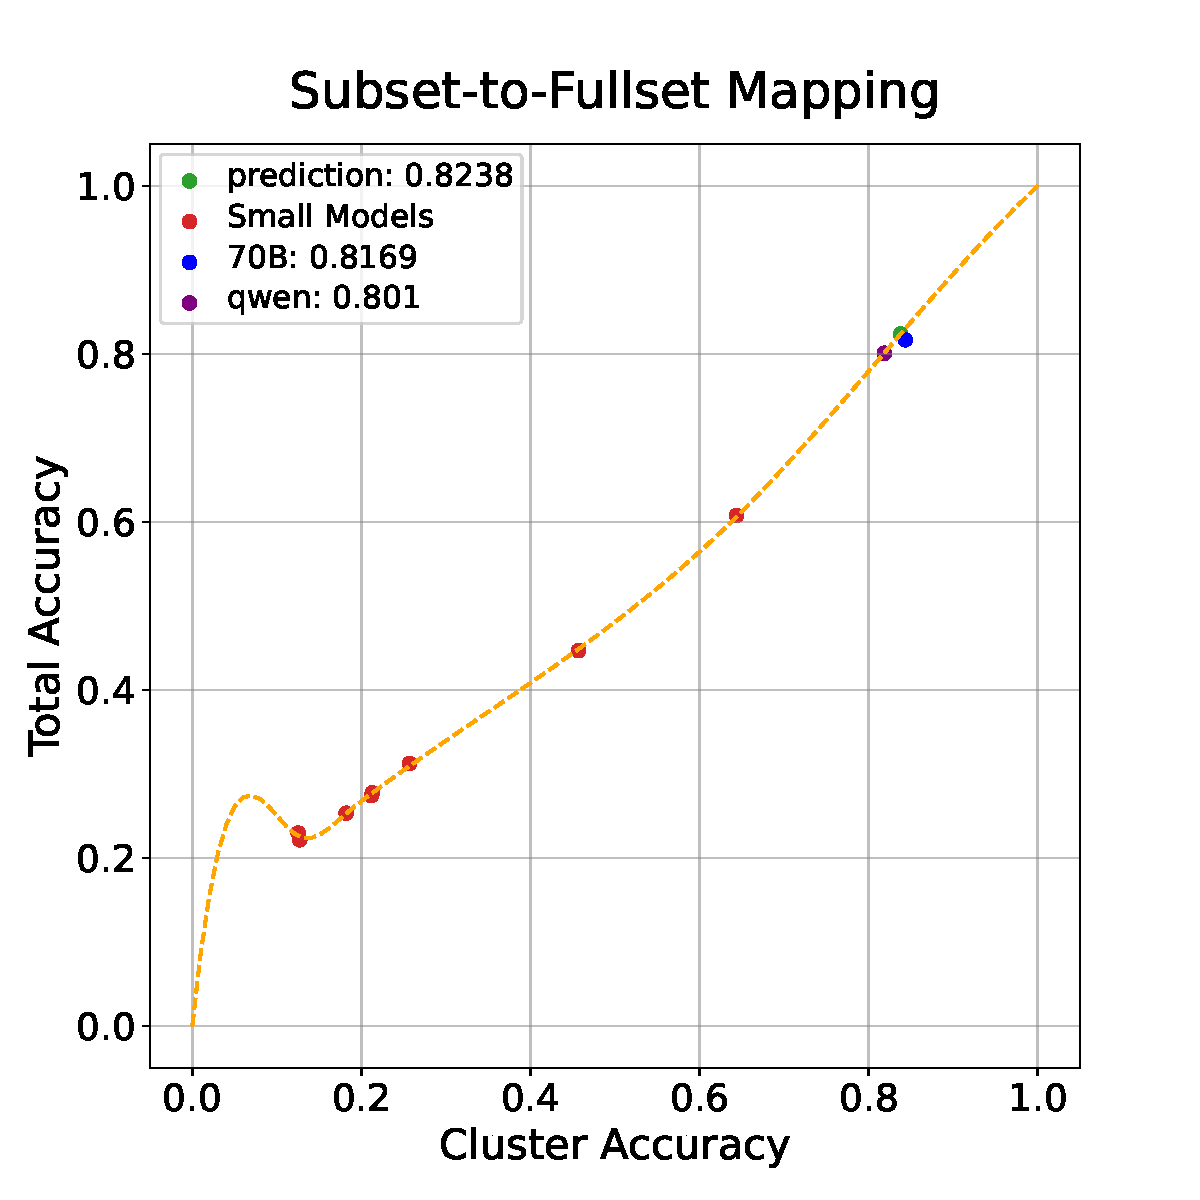
\includegraphics[width=\linewidth]{figures/experiments/mapping/BBH_0.0025_qwen_acc.pdf}
        \caption{$T=0.0025$}\label{subfig:bbh_0.0025}
    \end{subfigure}% 关键：加%取消换行符的隐形空格
    \hfill% 自动填充间距，无固定数值
    \begin{subfigure}[b]{0.22\textwidth}\centering
        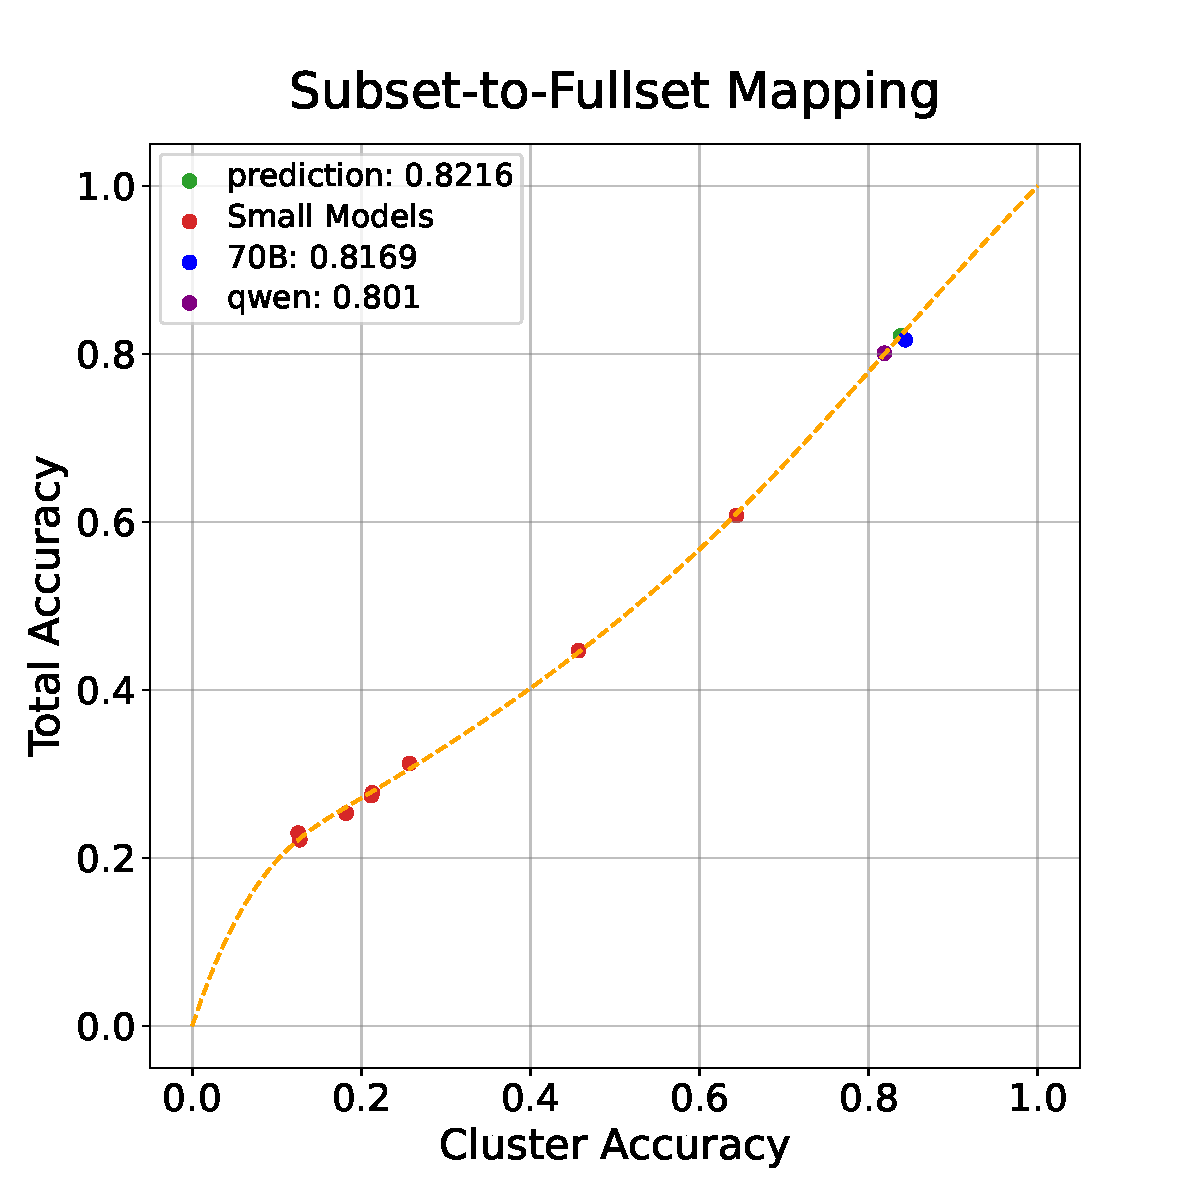
\includegraphics[width=\linewidth]{figures/experiments/mapping/BBH_0.005_qwen_acc.pdf}
        \caption{$T=0.005$}\label{subfig:bbh_0.005}
    \end{subfigure}%
    \hfill
    \begin{subfigure}[b]{0.22\textwidth}\centering
        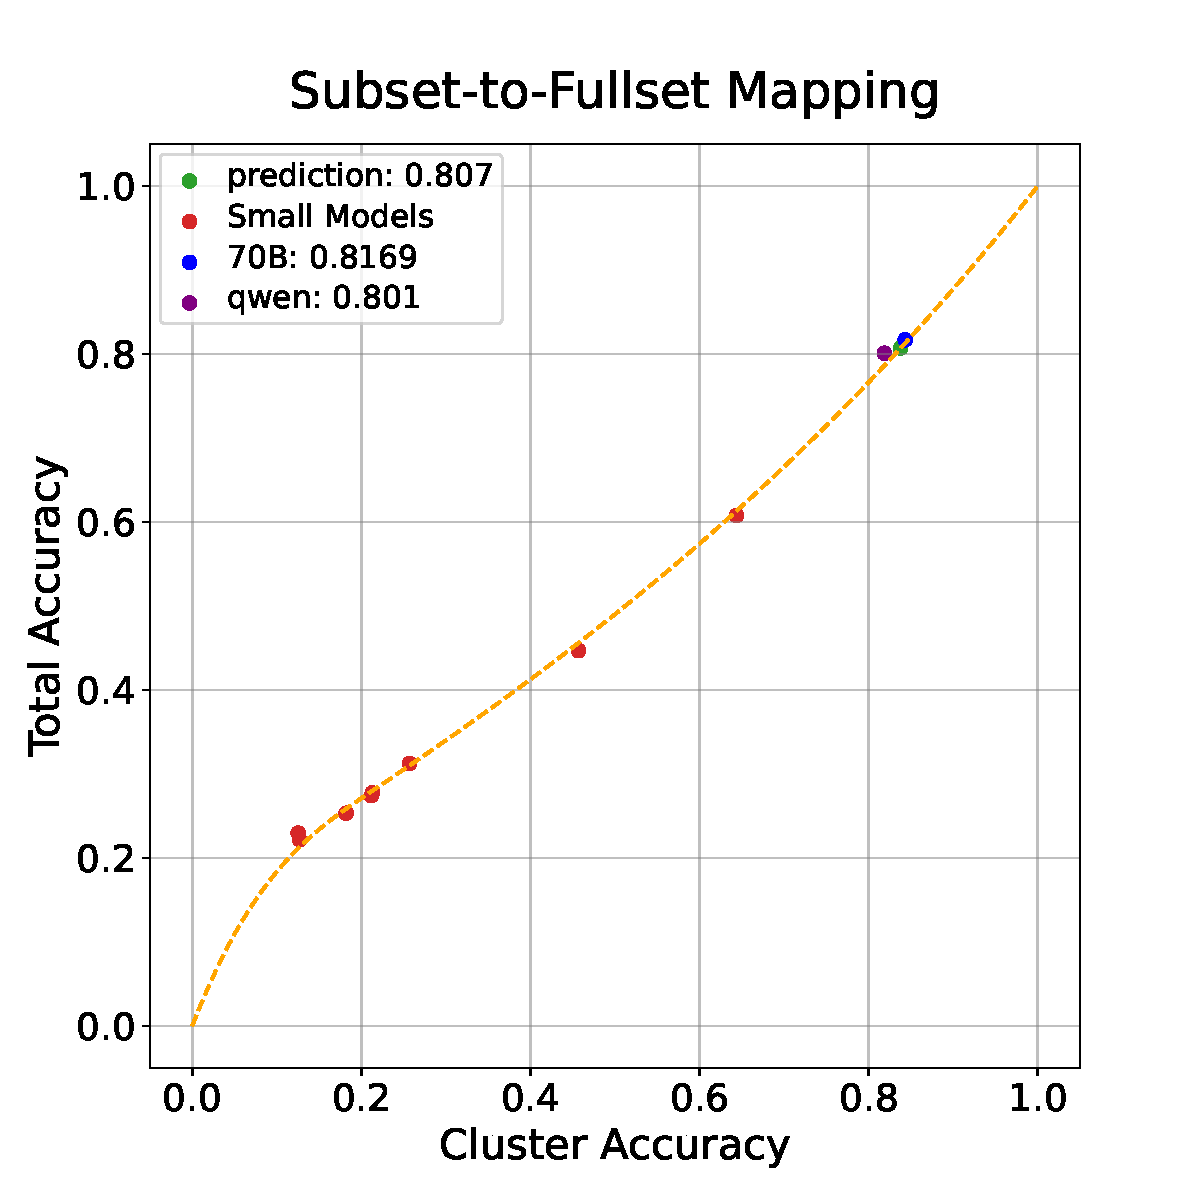
\includegraphics[width=\linewidth]{figures/experiments/mapping/BBH_0.01_qwen_acc.pdf}
        \caption{$T=0.01$}\label{subfig:bbh_0.01}
    \end{subfigure}%
    \hfill
    \begin{subfigure}[b]{0.22\textwidth}\centering
        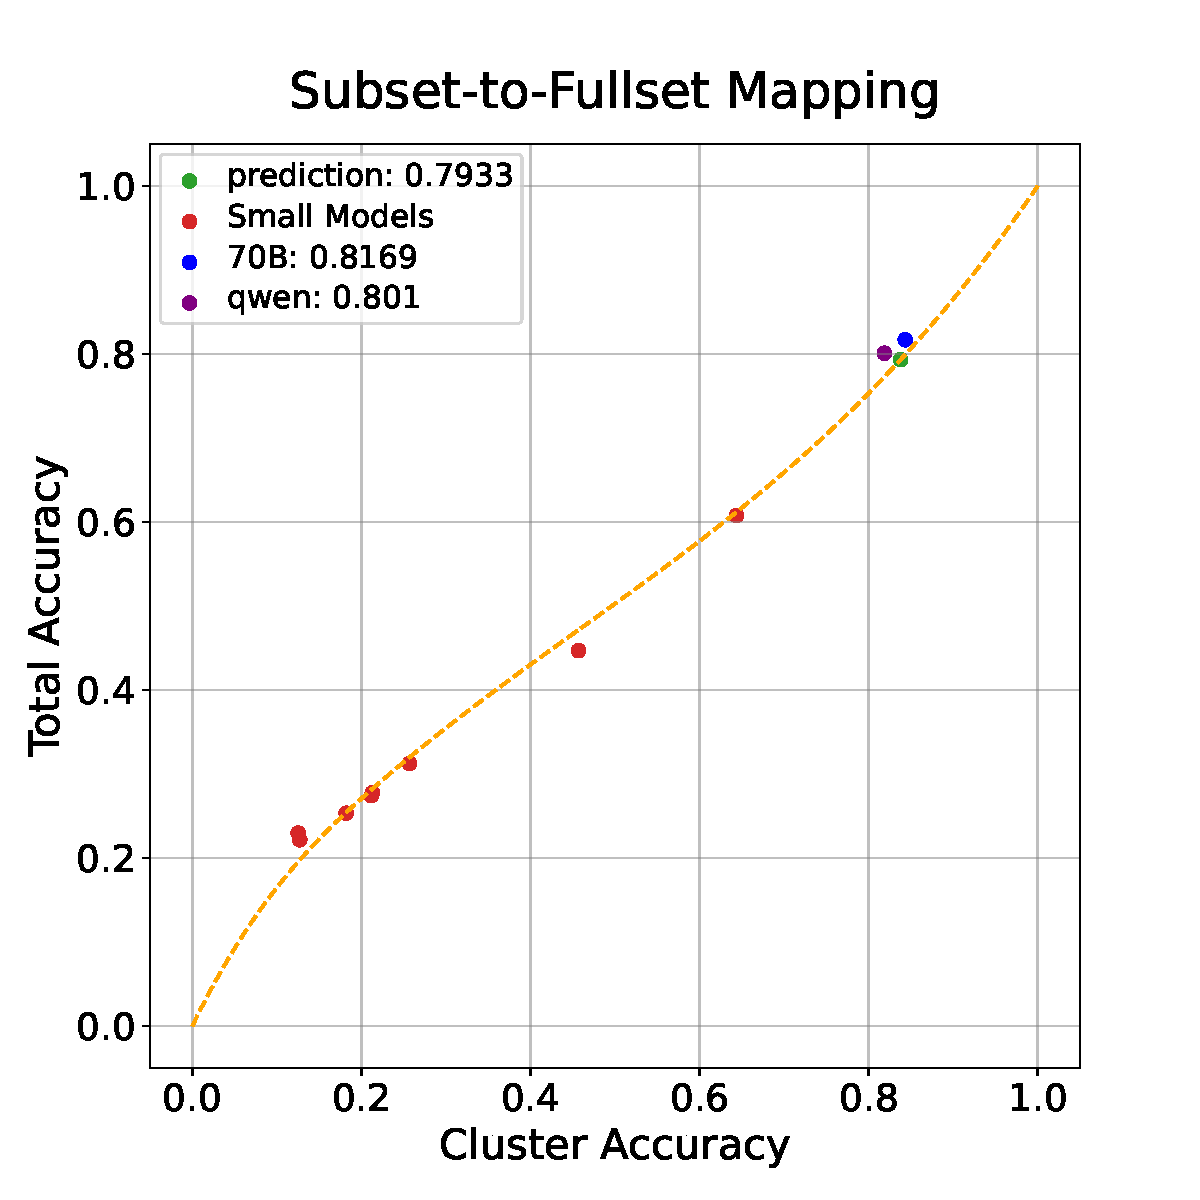
\includegraphics[width=\linewidth]{figures/experiments/mapping/BBH_0.02_qwen_acc.pdf}
        \caption{$T=0.02$}\label{subfig:bbh_0.02}
    \end{subfigure}
    
    \caption{Ablation of RMSE Threshold $T$.}
    \label{fig:RMSE_threshold}
    \vspace{-10pt}
\end{figure*}
% To evaluate different interpolation methods for prediction accuracy, we compared various mathematical approaches. Our baseline method uses quartic polynomial interpolation, which we compare against several alternative approaches, including Cubic spline interpolation, Cubic polynomial interpolation, and Quintic polynomial interpolation

% The comparative results across different benchmarks are shown in \cref{tab:interpolation_results}. We report the prediction error between the real performance of a large model and the mapping result.

% \begin{table}[!t]
% \caption{Comparison of different interpolation methods across benchmarks.}
% \centering
% \small
% \begin{tabular}{c|ccc}
% \toprule
% Prediction Error & BBH & Math & MMLU-pro \\
% \midrule
% Cubic Spline & 0.68 & 1.31 & 1.37 \\
% Cubic Polynomial & 3.38 & 1.12 & 1.35 \\
% Quintic Polynomial & 0.18 & 1.42 & 1.36 \\
% Quartic Polynomial & 1.77 & 1.28 & 1.35 \\
% \midrule 
% Smooth Spline & 2.51 & 0.35 & 0.03 \\
% \bottomrule
% \end{tabular}
% \label{tab:interpolation_results}
% \end{table}

% In \cref{fig:mappling_results_bbh}, we plot the mapping process using different interpolation formulas, where the x-axis represents the predictable subset indices and the y-axis represents the full set indices. The red points are the numerical values to be fitted, green points represent predicted values, purple points represent anchor points, and blue points show the actual performance.

% The prediction performance shows certain robustness across different interpolation methods. We aim to use the simplest possible interpolation function while maintaining low prediction errors. Based on the above results, we observe that the Cubic Polynomial shows larger prediction errors due to underfitting on BBH, while the Cubic Spline exhibits some overfitting. Both Quartic Polynomial and Quintic Polynomial perform well, therefore, we chose the Quartic Polynomial method as it requires fewer fitting parameters.
% \begin{figure}[!t]
%     \centering
%     \begin{minipage}{0.24\textwidth}
%         \centering
%         \includegraphics[width=\textwidth]{figures/experiments/mapping/cubic_spline.pdf}
%         % \caption*{Cubic Polynomial}
%     \end{minipage}
%     \begin{minipage}{0.24\textwidth}
%         \centering
%         \includegraphics[width=\textwidth]{figures/experiments/mapping/cubic_polynomial.pdf}
%         % \caption*{Quartic Polynomial}
%     \end{minipage}
%     \begin{minipage}{0.24\textwidth}
%         \centering
%         \includegraphics[width=\textwidth]{figures/experiments/mapping/quintic_polynomial.pdf}
%         % \caption*{Quintic Polynomial}
%     \end{minipage}
%     \begin{minipage}{0.24\textwidth}
%         \centering
%         \includegraphics[width=\textwidth]{figures/experiments/mapping/quartic_polynomial.pdf}
%         % \caption*{Cubic Spline}
%     \end{minipage}
%     \caption{Performance mapping with different interpolation methods on the BBH evaluation set. The cubic spline is overfitted, and the cubic polynomial method is underfitted. Quartic polynomials and quintic polynomials are comparable, while a quartic polynomial has fewer parameters.}
%     \label{fig:mappling_results_bbh}
% \end{figure}

% \labubu{When the number of small models used for fitting varies, the polynomial form also needs to be adaptively adjusted to ensure the robustness of the mapping. For instance, in the experiment of predicting the 12B model, the scaling function was adjusted from a quartic polynomial to a cubic polynomial to mitigate overfitting.}



\subsection{\labubu{Incorporating Anchor Point in Interpolation Mapping}}
\label{sec:anchor}
We find that the mapping relationship from predictable subset metrics to full evaluation set metrics is similar across models with different training data and architectures. This allows leveraging pre-trained models as "anchors" to refine the mapping and improve final estimation accuracy. \camera{In practice, we simply use an open-source model (Qwen2-72B)} as a refinement anchor. 
%and an in-house MoE model~\citep{lepikhin2020gshardscalinggiantmodels} with the same training data but different architecture (ID anchor). 
We first derive an interpolation curve using only small model metrics and fixed points $(0,0)$, $(1,1)$, then assess anchor compatibility. This shared mapping implies estimable subset metrics are highly correlated with full-set metrics and less prone to interference from other model parameters than loss-intermediate predictions.

We test two configurations:
\begin{itemize}[leftmargin=1.5em]
\item COD (w/o anchor): Full COD pipeline, but no anchor points in the mapping phase;
\item COD (w. anchor): COD method with Qwen2-72B as a refinement anchor;
% \item COD (w. ID anchor): COD with our in-house MoE model as an in-domain anchor.
\end{itemize}
\revise{We list the performance of anchor models and the target model in ~\cref{tab:anchor_info}.}
% 同时，我们在\cref{appdix:anchor_points} MATH与MMLU-pro两个评估集上对比了引入与不引入Anchor point参与Mapping的差异。MATH评估集在可外推子集与全集具有明显差异，添加Anchor point后显著提升了拟合与预测效果。而MMLU-pro评估集可预估子集占比高，可预估子集指标与全集基本接近，是否引入Anchor point差异不大。
\camera{In \cref{appdix:anchor_points}, we also compare the differences of using anchor points in the Mapping stage against not using them on two evaluation datasets: MATH and MMLU‑pro.
The MATH dataset shows a clear discrepancy between the predictable subset and the full set, and adding anchor points significantly improves the fitting and prediction performance.
In contrast, the MMLU‑pro dataset has a high proportion of predictable instances (listed in \cref{sec:ablation_extrapolation}), and its metrics for the predictable subset are close to those of the full set, so introducing anchor points yields little difference.}

\begin{table*}[h]
\centering
\caption{Performance comparison among the target model and anchor models.}
\label{tab:benchmark_results}
\resizebox{\textwidth}{!}{%
\begin{tabular}{lcccccccc}
\toprule
\textbf{Model} & \textbf{GSM8K} & \textbf{MATH} & \textbf{BBH} & \textbf{TriviaQA} & \textbf{MBPP} & \textbf{AGIEval} & \textbf{DROP} & \textbf{MMLU-pro} \\
\midrule
70B-Dense & 88.55 & 48.02 & 81.69 & 80.66 & 68.00 & 58.20 & 76.82 & 57.28 \\
Qwen2-72B & 88.63 & 53.08 & 80.10 & 84.23 & 71.60 & 64.16 & 77.56 & 56.93 \\
% 2.5B-MoE  & 86.66 & 50.36 & 79.60 & 72.17 & 70.60 & 58.70 & 74.30 & 57.37 \\
\bottomrule
\end{tabular}%
}
\label{tab:anchor_info}
\end{table*}

\begin{figure*}[!t]
    \centering
    \begin{subfigure}[b]{0.24\textwidth}\centering
        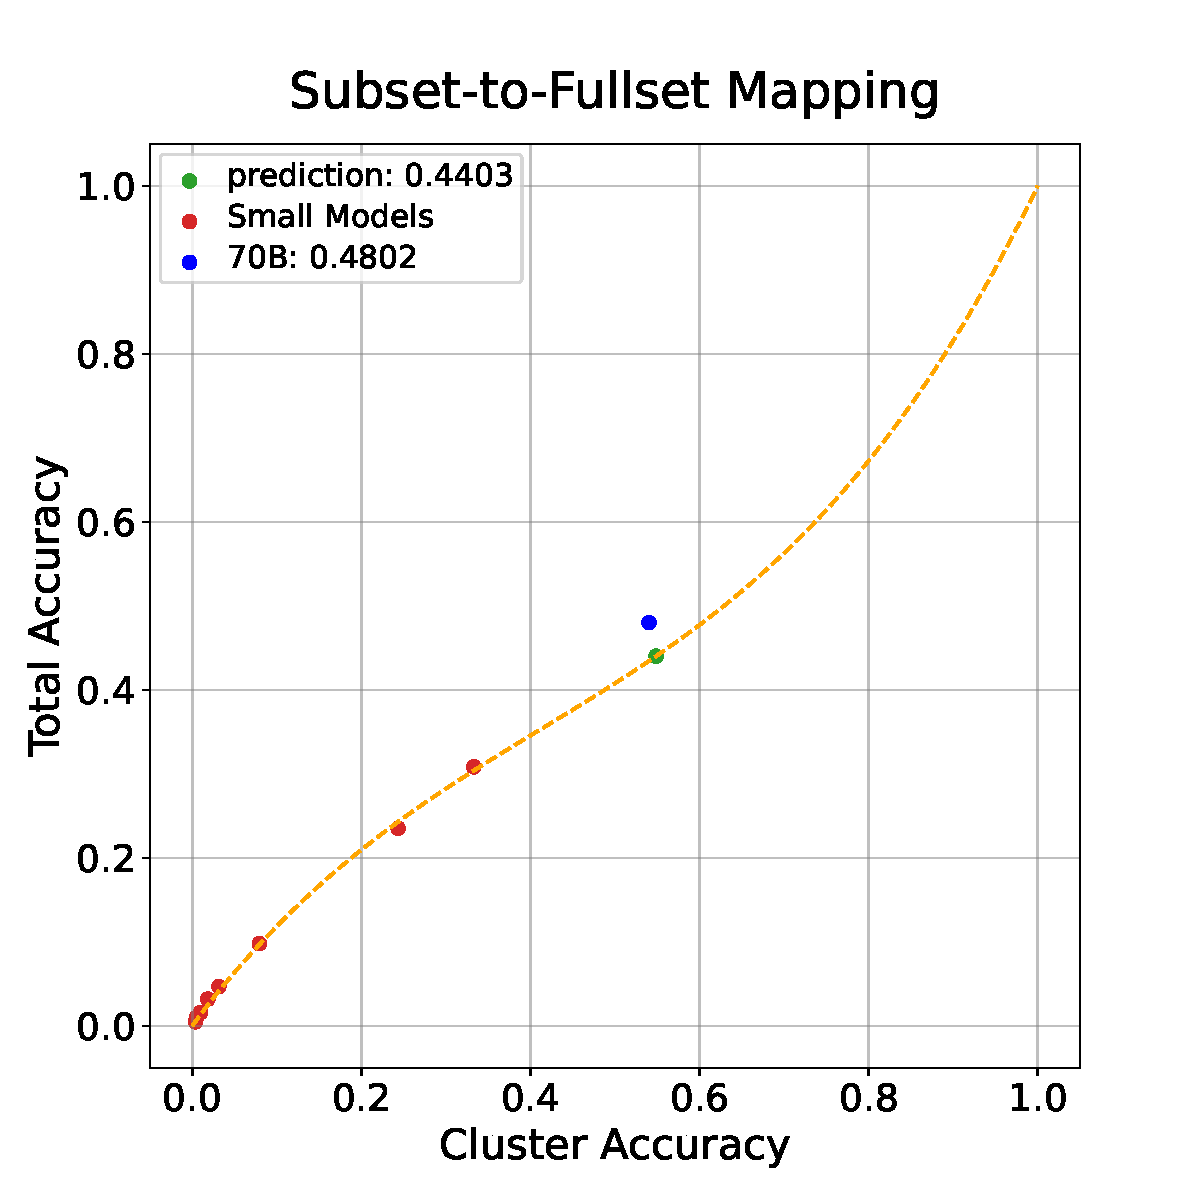
\includegraphics[width=\linewidth]{figures/experiments/mapping/MATH_0.005_None_acc.pdf}
        \caption{\small{MATH w/o anchor}}\label{subfig:bbh_0.0025}
    \end{subfigure}% 关键：加%取消换行符的隐形空格
    \hfill% 自动填充间距，无固定数值
    \begin{subfigure}[b]{0.24\textwidth}\centering
        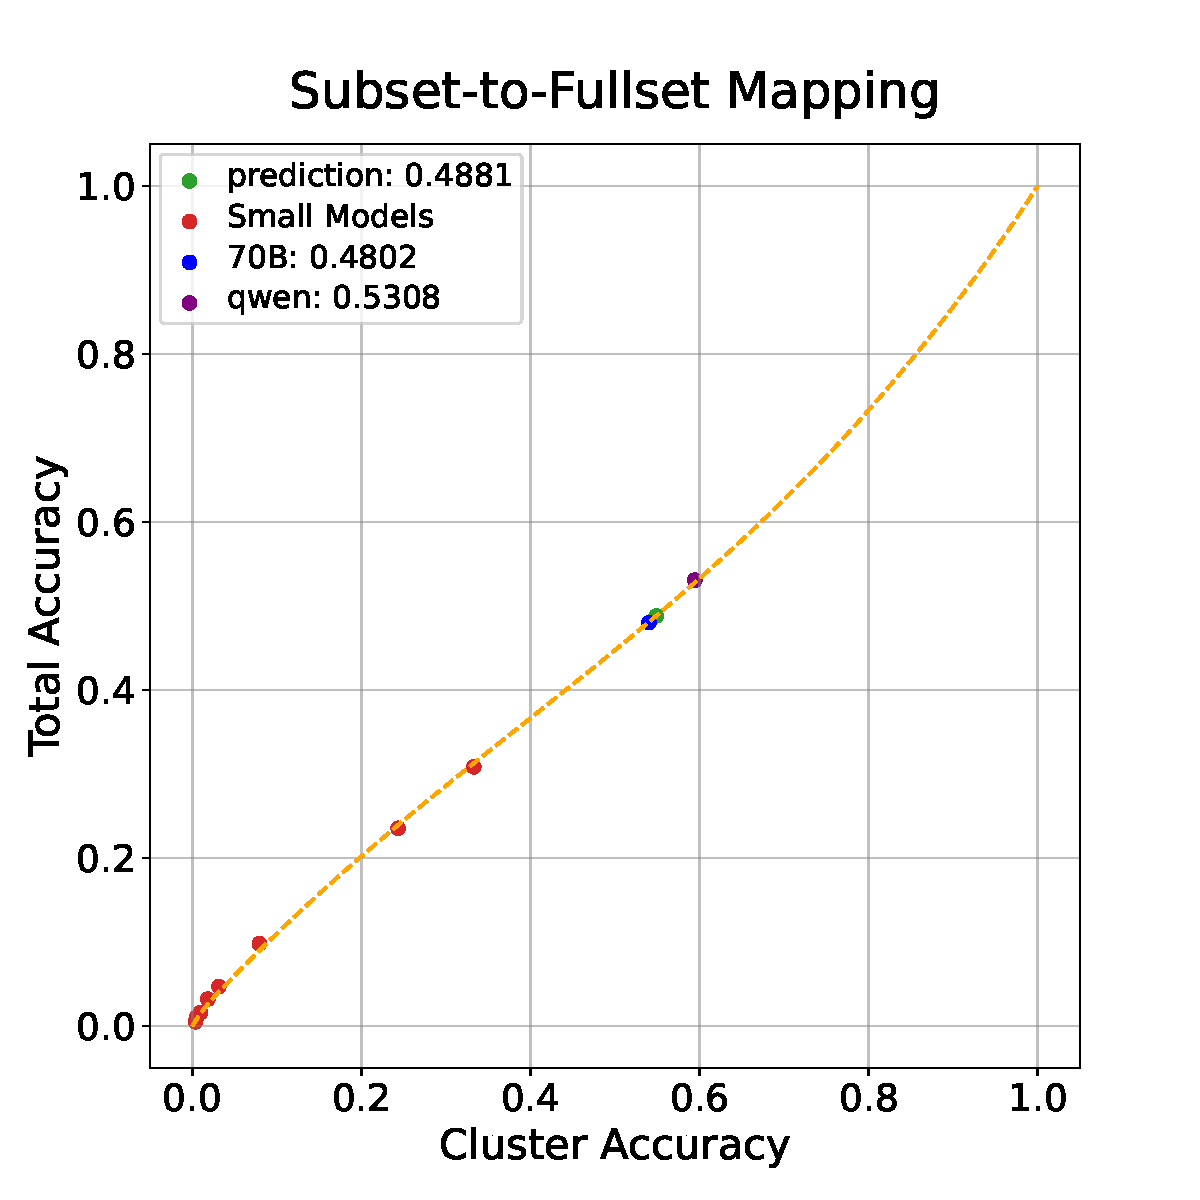
\includegraphics[width=\linewidth]{figures/experiments/mapping/MATH_0.005_qwen_acc.pdf}
        \caption{\small{MATH w/ anchor}}\label{subfig:bbh_0.005}
    \end{subfigure}%
    \hfill
    \begin{subfigure}[b]{0.24\textwidth}\centering
        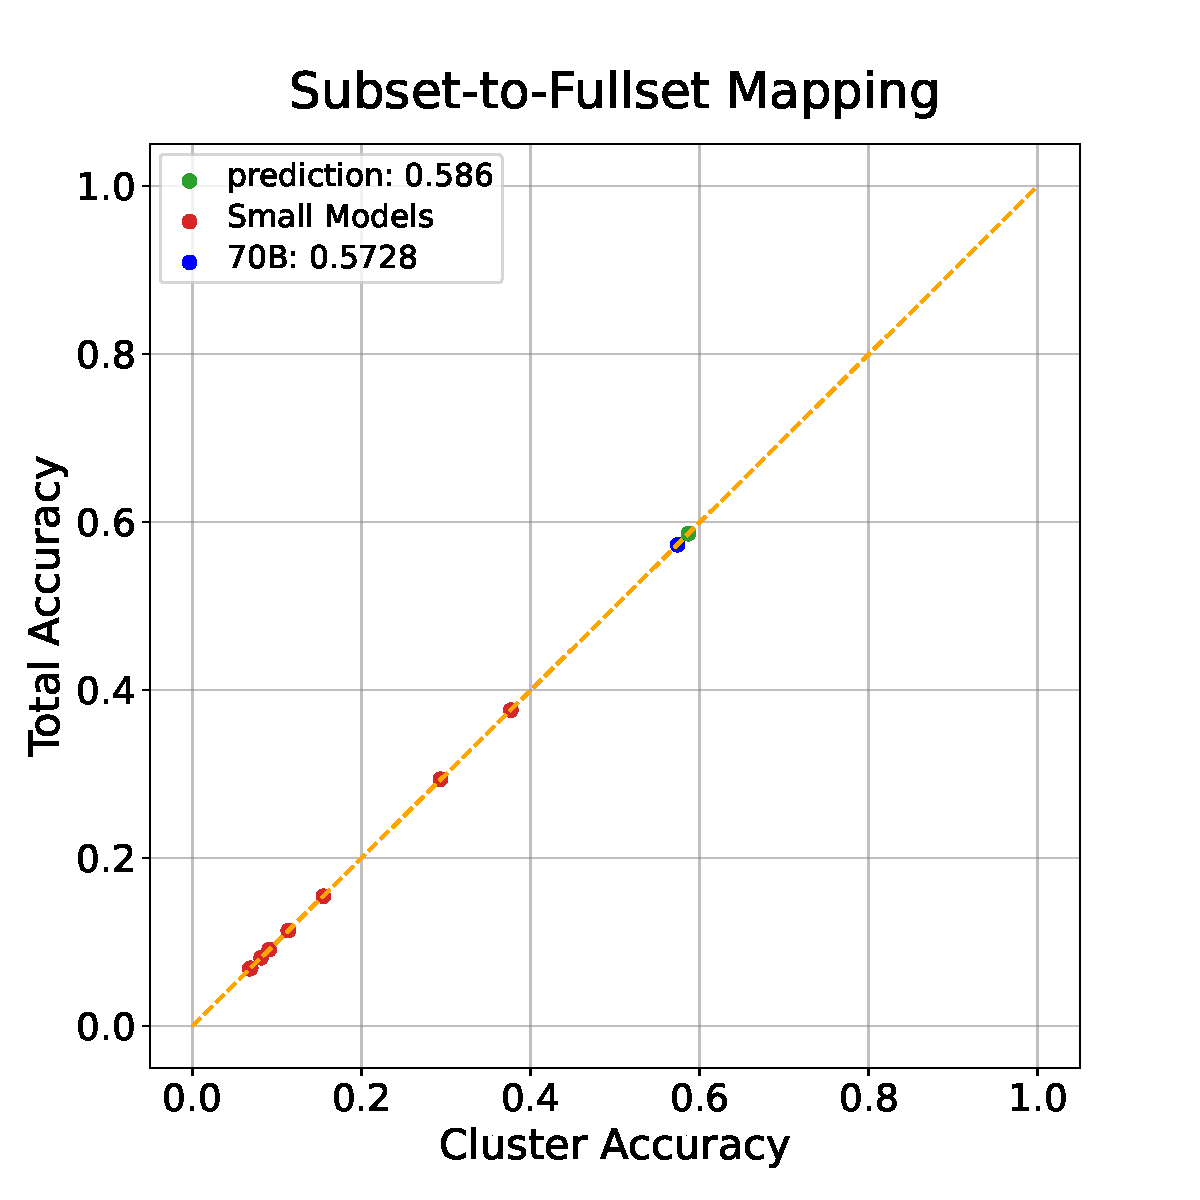
\includegraphics[width=\linewidth]{figures/experiments/mapping/MMLUpro_0.005_None_acc.pdf}
        \caption{\small{MMLUpro w/o anchor}}\label{subfig:bbh_0.01}
    \end{subfigure}%
    \hfill
    \begin{subfigure}[b]{0.24\textwidth}\centering
        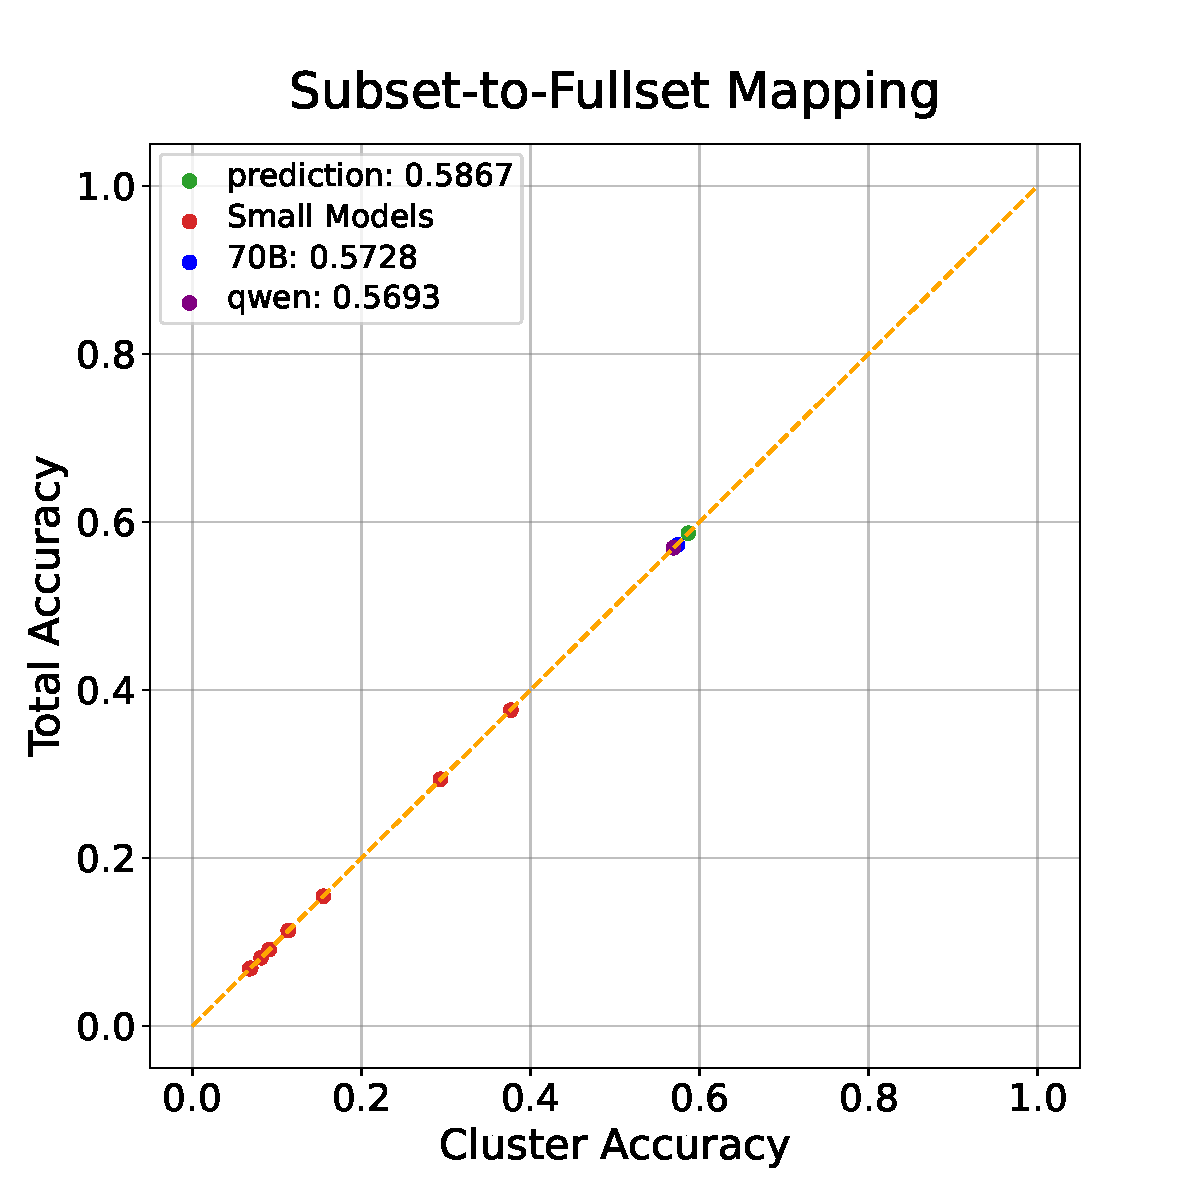
\includegraphics[width=\linewidth]{figures/experiments/mapping/MMLUpro_0.005_qwen_acc.pdf}
        \caption{\small{MMLUpro w/ anchor}}\label{subfig:bbh_0.02}
    \end{subfigure}
    \caption{\camera{Effectiveness of mapping with or without anchor points.}}
    \label{appdix:anchor_points}
\label{fig:anchor_compare}

\end{figure*}

\begin{table*}[]
\centering
\small
\caption{Influence of anchor points in the mapping stage on prediction error (\%). Errors < 2\% are considered accurate (green), while errors > 5\% are considered invalid (red). ↓ indicates lower is better.}
\setlength{\tabcolsep}{2.5pt}
\resizebox{\textwidth}{!}{% 自适应页面宽度
\begin{tabular}{c|c|cc|c*{7}{c}}
\toprule
\multirow{2}{*}{Setting} & \multirow{2}{*}{Method} & \multicolumn{2}{c|}{Overall} & \multicolumn{8}{c}{Individual Task Sets} \\
\cmidrule(lr){3-4} \cmidrule(lr){5-12}
& & Mean$\downarrow$ & Max$\downarrow$ & GSM8k & MATH & BBH & TriviaQA & MBPP & AGIEval & DROP & MMLU-pro \\

% & w. ID anchor & {1.63} & {2.38} & {2.23} & {1.28} & {1.77} & {1.64} & {2.19} & {2.38} & {0.23} & {1.35} \\
\midrule
\multirow{2}{*}{End-to-end(exp)} & w/o anchor & 3.10 & 6.00 & 4.00 & 3.86 & \greenhl{0.64} & \greenhl{0.68} & \greenhl{1.75} & \redhl{6.00} & 4.11 & 3.72 \\
& w/ anchor & 3.08 & 6.42 & \greenhl{0.56} & \redhl{5.75} & \greenhl{0.93} & 2.25 & 2.82 & \redhl{6.42} & \greenhl{1.10} & 4.80 \\
% & w/ ID anchor & 9.55 & 21.85 & 4.76 & 16.05 & 10.56 & 1.89 & 8.24 & 10.63 & 2.41 & 21.85 \\
\midrule
\multirow{2}{*}{End-to-end(BNSL)} & w/o anchor & 5.17 & 13.05 & 4.23 & \redhl{5.88} & \redhl{13.05} & \redhl{5.86} & 2.55 & \greenhl{0.82} & \greenhl{1.53} & \redhl{7.42} \\
& w/ anchor & 3.60 & 6.65 & \greenhl{0.18} & \redhl{5.77} & \greenhl{1.28} & 4.17 & 4.22 & \redhl{6.65} & \greenhl{1.43} & \redhl{5.10} \\
% & w/ ID anchor & 15.34 & 30.49 & 6.32 & 24.04 & 14.25 & 5.72 & 15.86 & 15.99 & 10.06 & 30.49 \\
\midrule
\multirow{2}{*}{COD} & w/o. anchor & 2.65 & 4.98 & 3.10 & 3.99 & \greenhl{0.97} & 2.38 & \greenhl{1.59} & 4.98 & 2.86 & \greenhl{1.32} \\
& w. anchor & \textbf{1.55} & \textbf{2.68} & 2.68 & \greenhl{0.79} & \greenhl{0.47} & \greenhl{1.97} & 2.42 & \greenhl{1.64} & \greenhl{1.05} & \greenhl{1.39} \\
\bottomrule
\end{tabular}}
\label{tab:ablation_study}
% \vspace{-10pt}
\end{table*}

% %我们同样给End-to-end与BNSL等Baseline方法添加anchor point作为对照，添加的OOD与ID anchor都与COD方法相同。在实践中，我们把anchor point直接参与拟合外推公式。
% \cref{tab:ablation_study} shows that COD method incorporating either OOD or ID anchors consistently enhances prediction accuracy. 
% % 然而End-to-end与BNSL等基线方法并没有从添加anchor point中取得提升。
% This suggests a stable correlation between predictable subset and full-set metrics across diverse models, enabling the use of existing model evaluations to improve predictions for new models. 
% % 相对的，End-to-end与BNSL只能把anchor point作为拟合点，仅能让预测目标靠近anchor point的Scaling趋势，但不同训练数据和结构训练的模型Scaling趋势具有显著差异，在不同能力分向上表现差异性大，从而无法获取有效预估。
% Furthermore, since our clustering identifies intrinsic properties of evaluation sets, the derived predictable subsets are applicable to new models. Additional ablations on the interpolation method (\cref{sec:interpolation_ablation}) confirms quartic functions are suitable.

\camera{To facilitate a direct comparison, we also apply the anchor point to baseline methods including End-to-end(exp) and End-to-end(BNSL), using the same anchor as in the COD method. In practice, the anchor points are directly incorporated into the fitting process of the extrapolation formula.}

\camera{\cref{tab:ablation_study} shows that the COD method incorporating anchor consistently enhances prediction accuracy. However, the End-to-end(exp) and End-to-end(BNSL) baselines failed to derive any benefit from the addition of anchor points. 
This suggests a stable correlation between the predictable subset and full-set metrics across diverse models, enabling the use of existing model evaluations to improve predictions for new models. 
In contrast, End-to-end(exp) and End-to-end(BNSL) treat anchor points merely as fitting samples, aligning the prediction target solely with the scaling trend of the anchors. 
Yet, scaling trends differ significantly across models trained on different data and architectures, manifesting as high variance across different capability dimensions; consequently, these methods fail to produce effective estimations. 

Furthermore, since our clustering identifies intrinsic properties of evaluation sets, the derived predictable subsets are applicable to new models.}
% Additional ablations on the interpolation method (\cref{sec:interpolation_ablation}) confirm that quartic functions are suitable.





\section{Experimental Settings and Training Recipe}
\label{append:setting}
\noindent\textbf{Training recipe.}
To establish performance predictions for large language models, we conduct systematic experiments with a suite of smaller-scale models across different parameter counts. All our models are trained from scratch on a corpus of text data. We do not fix the data budget for all models; instead, we maintain a consistent Data-to-CPT (Compute Per Token) ratio for all models, as mentioned in \cref{sec:exp_setups}. We list model configurations in \cref{tab:model_configs_dense}.

We adopt the in-house training data that comprises multilingual text corpora, with increased weighting for domains such as STEM, code, and general knowledge, following Llama3~\citep{grattafiori2024llama}, Deepseek-v2~\citep{liu2024deepseek}, Fineweb-EDU~\citep{lozhkov2024fineweb}, etc. We apply several de-duplication methods and data cleaning mechanisms to each data source to ensure high-quality tokens.

The model architecture is consistent with Llama3.1~\citep{grattafiori2024llama}, incorporating Grouped-Query Attention (GQA)~\citep{ainslie2023gqa}, SwiGLU activation function~\citep{shazeer2020glu}, RMSNorm~\citep{zhang2019root} with Pre-normalization, etc. The models are trained using $BF16$ precision with a sequence length of $8192$ and a RoPE~\cite{su2024roformer} base of $500,000$. We employ the AdamW optimizer with $\beta=(0.9,0.95)$, a weight decay of $0.1$, and a dropout rate of $0.1$.

All models are trained on a constant learning rate scheduler with a few-step warmup stage. To determine the learning rate and batch size, we adopt the hyperparameter scaling laws from \citet{liu2024deepseek}. Specifically, the optimal learning rate $\eta_{\mathrm{opt}}$, and the optimal batch size $B_{\mathrm{opt}}$ are defined as power laws of the compute, measured in FLOPs: $\eta_{opt}=a_1\cdot C^{-b_1}$ and $B_{opt}=a_2\cdot C^{b_2}$, where $a_1$, $b_1$, $a_2$, $b_2$ are parameters to be fitted. We perform a grid search on our small models to identify their optimal learning rates and batch sizes, and then extrapolate these findings to the bigger models.
% \noindent\textbf{Model Specifications}

\begin{table}[!t]
\centering
\small
\caption{Model architecture specifications across different sizes.}
\setlength{\tabcolsep}{2.5pt}
\begin{tabular}{c|ccccccccc}
\toprule
 & 122M & 238M & 411M & 652M & 973M & 1.9B & 7B & 12B & 70B (Target) \\
\midrule
Param. (M) & 122 & 238 & 411 & 652 & 973 & 1,901 & 6,980 & 12,022 & 68,452 \\
Compute Per Token (B) & 1.535 & 2.684 & 4.275 & 6.378 & 9.060 & 16.436 & 54.761 & 91.609 & 475.131 \\
Tokens (B) & 26 & 45 & 72 & 108 & 153 & 277 & 923 & 1,544 & 8,012 \\
Continue-Trained Tokens (B) & 3 & 5 & 8 & 12 & 18 & 33 & 114 & 191 & 1,000 \\
Model Dimension & 1,024 & 1,280 & 1,536 & 1,792 & 2,048 & 2,560 & 4,096 & 4,608 & 8,192 \\
FFN Dimension & 3,584 & 4,480 & 5,376 & 6,272 & 7,168 & 8,960 & 14,336 & 16,128 & 28,672 \\
Heads & 8 & 10 & 12 & 14 & 16 & 20 & 32 & 36 & 64 \\
KV Heads & 8 & 10 & 12 & 14 & 16 & 20 & 8 & 12 & 8 \\
\bottomrule
\end{tabular}
\label{tab:model_configs_dense}
\end{table}

\anno{\noindent\textbf{Training Resources.} The 7B dense model is trained on 923B tokens, consuming 52,800 H800 GPU-hours. The computational resources used for the other models can be estimated proportionally based on their respective compute requirements.}

\anno{\noindent\textbf{Evaluation settings and protocol.}}
We conducted performance scaling estimation experiments across eight major LLM evaluation sets. These evaluation sets span a diverse range of capabilities, including Math, Reasoning, Knowledge, Coding, Reading, and general abilities. All pretrained LLMs were evaluated using a few-shot methodology to obtain the performance metrics. Detailed information is provided in~\cref{tab:evaluation_info}. \anno{Our evaluation methodology aligns with that used for the Llama3~\citep{grattafiori2024llama} pre-trained models. We assess the models' capabilities directly through few-shot text completion tasks without any instruction tuning or Supervised Fine-Tuning (SFT). This evaluation method is chosen because even a small amount of SFT data can significantly influence performance on downstream tasks, thereby not reflecting the inherent capabilities of the pre-trained model itself.}

\anno{\noindent\textbf{Software Framework.}
All models are trained using the Megatron framework. The evaluation code is an in-house implementation designed to be consistent with the Llama3~\citep{grattafiori2024llama} evaluation methodology.}

\label{appix:exp_settings}
\begin{table}
\centering
\small
\caption{Information of evaluation datasets.}
\setlength{\tabcolsep}{3pt}
\begin{tabular}{c|ccc}
\toprule
Dataset & Domain & \#Questions & \#Shots \\
\midrule
GSM8K & Math & 1,319 & 8 \\
MATH & Math & 5,000 & 4 \\
BBH & Reasoning & 6,511 & 3 \\
TriviaQA & Knowledge & 17,944 & 5 \\
MBPP & Coding & 500 & 3 \\
AGIEval& Comprehensive & 8,063 & 5 \\
DROP & Reading & 9,536 & 3 \\
MMLU-pro  & Comprehensive & 12,032 & 5 \\
\bottomrule
\end{tabular}
\label{tab:evaluation_info}
\end{table}

% \renewcommand{\thefigure}{D\arabic{figure}}
% \renewcommand{\thetable}{D\arabic{table}}
% \renewcommand{\theproposition}{D.\arabic{proposition}}
% \setcounter{table}{0} 
% \setcounter{figure}{0} 

% \section{Additional Prediction Results for a Medium-size Model}
% \label{append:12B}
% \anno{The COD method is also effective for predicting the capabilities of medium-size language models. To demonstrate this, we conducted an experiment to predict the performance of a 12B model using source models ranging from 122M to 1.9B parameters. This setup maintains a similar ~6$\times$ parameter-size ratio as our main experiment (predicting 70B from models up to 12B).

% For this experiment, clustering relied exclusively on the passrate@100 data from the 122M to 1.9B source models to prevent data leakage from the target model. The results in~\cref{tab:12B_results} show that COD is more robust and less demanding on the size of source models compared to the baselines. For instance, the baseline methods perform poorly on the BBH benchmark, In contrast, COD accurately captures the trend of accuracy growth as compute increases and yields precise extrapolations. We will include a plot of this curve in the main text to visually demonstrate the clear advantage of COD.

% The prediction errors of all methods for the 12B model are significantly higher than those for the 70B model reported in~\cref{subsec:Prediction_Experiments}. Extrapolation accuracy improves when larger source models are employed for fitting, as a greater number of samples have ``emerged''. If the largest source model is excessively small, numerous samples remain ``unemerged'', resulting in substantial errors when extrapolating to a significantly larger model.}

% \begin{table*}[!t]
% \small
% \setlength{\tabcolsep}{1.8pt} % 保持原列间距设置
% \centering
% \caption{Absolute prediction error (\%) on evaluation sets for predicting the performance of the 12B model. Errors < 2\% are considered accurate (green), while errors > 5\% are considered invalid (red). $\downarrow$ indicates lower is better.}
% \begin{tabular}{c|c|cc|cc|cc|cc} % 列结构：任务/指标 | 真值 | 4组[Prediction|Error]
% \toprule
% \multirow{2}{*}{Task Sets/Metrics} & \multirow{2}{*}{Ground Truth} & \multicolumn{2}{c|}{\textbf{Loss-intermediate}} & \multicolumn{2}{c|}{\textbf{End-to-end}} & \multicolumn{2}{c|}{\textbf{BNSL}} & \multicolumn{2}{c}{\textbf{COD}} \\
% \cmidrule(lr){3-10} % 分隔线覆盖所有方法的Prediction-Error列
% & & Prediction & Error & Prediction & Error & Prediction & Error & Prediction & Error \\
% \toprule
% \multicolumn{10}{c}{\textbf{Overall Metrics}} \\ % 横向标题适配10列
% \midrule
% Mean & - & - & 14.92 & - & 10.52 & - & 17.42 & - & \textbf{4.68} \\
% Max & - & - & 23.82 & - & 24.43 & - & 28.26 & - & \textbf{10.39} \\
% \midrule
% \multicolumn{10}{c}{\textbf{Individual Task Sets}} \\ % 横向标题适配10列
% \midrule
% GSM8k & 70.47 & 60.86 & \redhl{9.61} & 63.66 & \redhl{6.81} & 80.99 & \redhl{10.52} & 60.08 & \redhl{10.39} \\
% MATH & 30.85 & 41.53 & \redhl{10.68} & 34.36 & 3.51 & 49.26 & \redhl{18.41} & 28.48 & 2.37 \\
% BBH & 60.76 & 36.94 & \redhl{23.82} & 36.33 & \redhl{24.43} & 36.10 & \redhl{24.66} & 57.751 & 3.05 \\
% TriviaQA & 58.84 & 68.42 & \redhl{9.57} & 59.88 & \greenhl{1.04} & 87.10 & \redhl{28.26} & 57.92 & \greenhl{0.93} \\
% MBPP & 47.80 & 28.53 & \redhl{19.27} & 36.51 & \redhl{11.29} & 27.95 & \redhl{19.85} & 44.50 & 3.30 \\
% AGIEval & 44.13 & 33.91 & \redhl{10.22} & 35.40 & \redhl{8.74} & 34.12 & \redhl{10.01} & 47.53 & 3.40 \\
% DROP & 54.35 & 35.05 & \redhl{19.30} & 37.19 & \redhl{17.16} & 36.73 & \redhl{17.62} & 63.50 & \redhl{9.14} \\
% MMLU-pro & 37.60 & 20.74 & \redhl{16.86} & 26.41 & \redhl{11.20} & 27.59 & \redhl{10.01} & 42.42 & 4.82 \\
% \bottomrule
% \end{tabular}
% \label{tab:12B_results}
% % \vspace{-10pt}
% \end{table*}


\section{Performance Prediction for Continue-Pretrained LLMs}
\label{sec:ppct}
Leading industry pre-trained LLMs (e.g., Deepseek-v3~\citep{deepseekai2025deepseekv3technicalreport}, Llama3~\citep{grattafiori2024llama}, Qwen-2.5~\citep{qwen2.5}) adopt the Continual Training (CT) strategy of concentrating high-quality data towards the end of the pre-training process. This phase is typically accompanied by learning rate decay, enabling the model to fully absorb this high-quality data. Due to significant changes in data distribution and the learning rate schedule, this approach often yields substantial improvements in metrics. Predicting a large model's final capability based solely on its performance during a ``stable'' phase with consistent data distribution does not reflect its ultimate capability. Therefore, we supplement this by providing metric predictions for the high-quality CT phase.

The relationship between model parameter scale and the volume of CT tokens is listed in~\cref{tab:model_configs_dense}. We conduct the same COD pipeline for CT models. We control the data distribution of the stable and decay phases for various smaller models, as well as their token-to-parameter ratio, to be consistent with the large model targeted for prediction. The last checkpoint is used for evaluation. Based on prior clustering labels, we perform fitting, extrapolation, and mapping to obtain the predicted performance for the large model. 

\begin{table}[!h]
\centering
\caption{Predicted vs. actual metrics for an LLM with 70B parameters after high-quality continued pretraining. Errors < 2\% are considered accurate (green)}
\label{tab:ct_results}
\begin{tabular}{lccc}
\toprule
Evaluation Set & Predicted Metric & Actual Metric & Prediction Error \\
\midrule
GSM8k          &    93.10        & 91.81         &    \greenhl{1.29}        \\
MATH           &    56.35        & 52.68         &    3.67         \\
BBH            &    83.05       &  85.32         &    2.27          \\
TriviaQA       &    79.29        & 84.05         &    4.76          \\
MBPP           &    72.42        & 73.20         &    \greenhl{0.78}          \\
AGIEval        &    63.22        & 64.18         &    \greenhl{0.96}          \\
DROP           &    82.34        & 81.39         &    \greenhl{0.95}          \\
MMLU-pro       &    62.11        & 59.34         &    2.77          \\
\bottomrule
\end{tabular}
\end{table}



% 我们注意到MATH, GSM8k与TriviaQA具有相对较大的预测误差，并认为造成预测不准确的原因可能有两类：
% 1. CT数据与评估集具有明显相关性，例如数学类评估集，少量训练即可带来大量指标提升。此时小模型指标的波动性较大，同时大模型能力上限也更收到训练数据质量约束，导致Scaling规律发生变化。
% 2. CT数据具有偏向性，部分评估集不能从中获得效果提升，例如TriviaQA, 让CT阶段前后的指标为波动关系，降低了小模型指外推的准确性。

Results listed in~\cref{tab:ct_results} show that the proposed COD method achieves an average prediction error of \camera{2.18}\%. We observe that MATH and TriviaQA exhibit relatively large prediction errors. We hypothesize that there are two main categories of reasons for this inaccuracy:

\begin{enumerate}[label=\arabic*.,leftmargin=1.5em]
    \item The CT data and the evaluation sets possess a significant correlation. For example, in math-related evaluation sets, a modest amount of training can yield substantial improvements in performance metrics. In such scenarios, the metrics for smaller models tend to show greater volatility and have inaccurate evaluations.
    \item The CT data exhibits inherent distribution bias, such that certain evaluation sets, such as TriviaQA, do not derive performance gains from it. This leads to potential significant fluctuations in the metrics after the CT phase, thereby diminishing the accuracy of extrapolating to larger models.
\end{enumerate}


\section{Difficulty Distribution of Predictable Subset}
\label{sec:difficulty_distribution}
% 我们观察在不同难度层级上的可预估子集任务占比，我们把不同评估集的可预估子集与全集的难度分布绘制在了~\cref{fig:diff_dist}中。我们采用12B模型的得分做为难度分级的依据。可以看出，在MMLU-pro, GSM8k评估集上，可预估子集占比较大。说明该评估集大部分题目Scaling性质良好。而在Math评估集上，很多得分接近0的困难题目不在可预估子集中，这部分题目的预估则需要Mapping阶段进行修正。同时BBH在各个难度分布上可预估子集的占比接近，这是因为BBH有部分题目随Compute提升的提升收益较小，表现出震荡走势。

% 我们可以通过可预估子集的占比来评估测试集质量。对于可预估子集占比更大的评估集，我们在小模型上进行的实验结论会更加可靠。
% 同时在我们构建评估集时，对不可预估类簇进行筛查或补充。保证每一类难度特征题目的最小数量，以此降低指标波动性。
We analyze the proportion of predictable subset tasks across different difficulty levels. 
The difficulty distributions of predictable subset versus complete sets for different evaluation benchmarks are illustrated in \cref{fig:diff_dist}. 
We use the scores from the 12B model as the basis for difficulty classification. 
The results show that MMLU-pro and GSM8k evaluation sets have larger proportions of predictable subsets, indicating that most questions in these datasets exhibit good performance scaling properties. In contrast, many difficult questions with near-zero scores in the MATH evaluation set fall outside the predictable subset, requiring adjustment during the mapping phase. 
Meanwhile, BBH exhibits consistent proportions of its predictable subset across varying difficulty levels, as some questions display oscillatory patterns with limited improvement, even with increased computational resources.


The proportion of the predictable subset can serve as a metric for assessing evaluation set quality. Evaluation sets with larger predictable subsets yield more reliable experimental conclusions from smaller models. When constructing evaluation sets, we recommend screening or supplementing unpredictable clusters and ensuring a minimum number of questions for each difficulty feature to reduce metric volatility.

\begin{figure}[htbp]
    \centering
    % First row
    \begin{minipage}{0.24\textwidth}
        \centering
        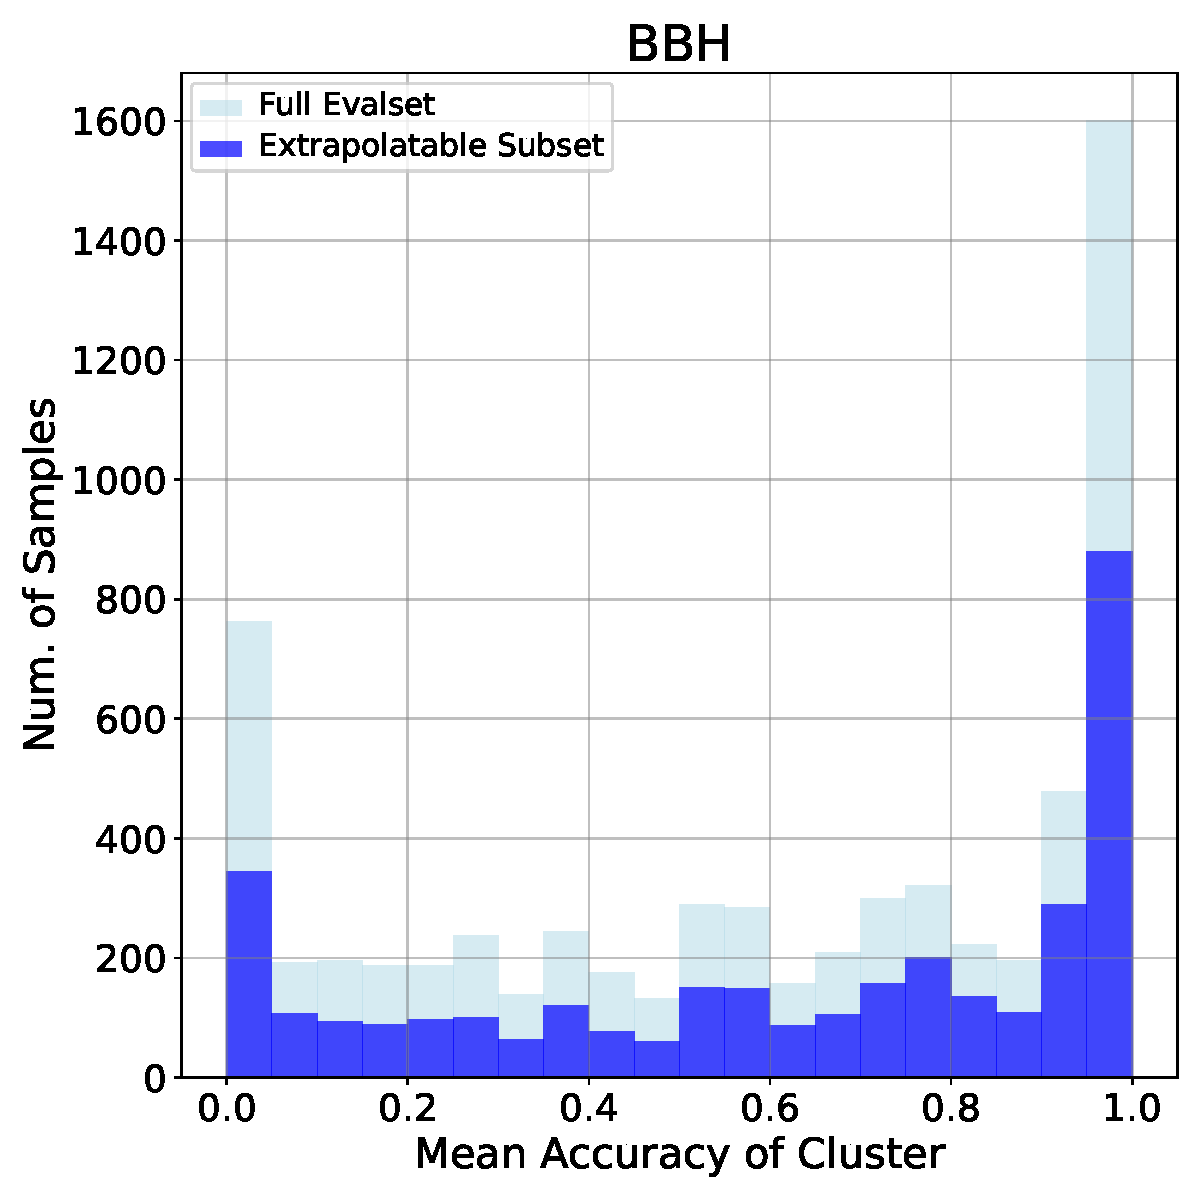
\includegraphics[width=\textwidth]{figures/appendix/difficulty_distributions/bbh.pdf}
        % \caption*{Title 1}
    \end{minipage}
    \begin{minipage}{0.24\textwidth}
        \centering
        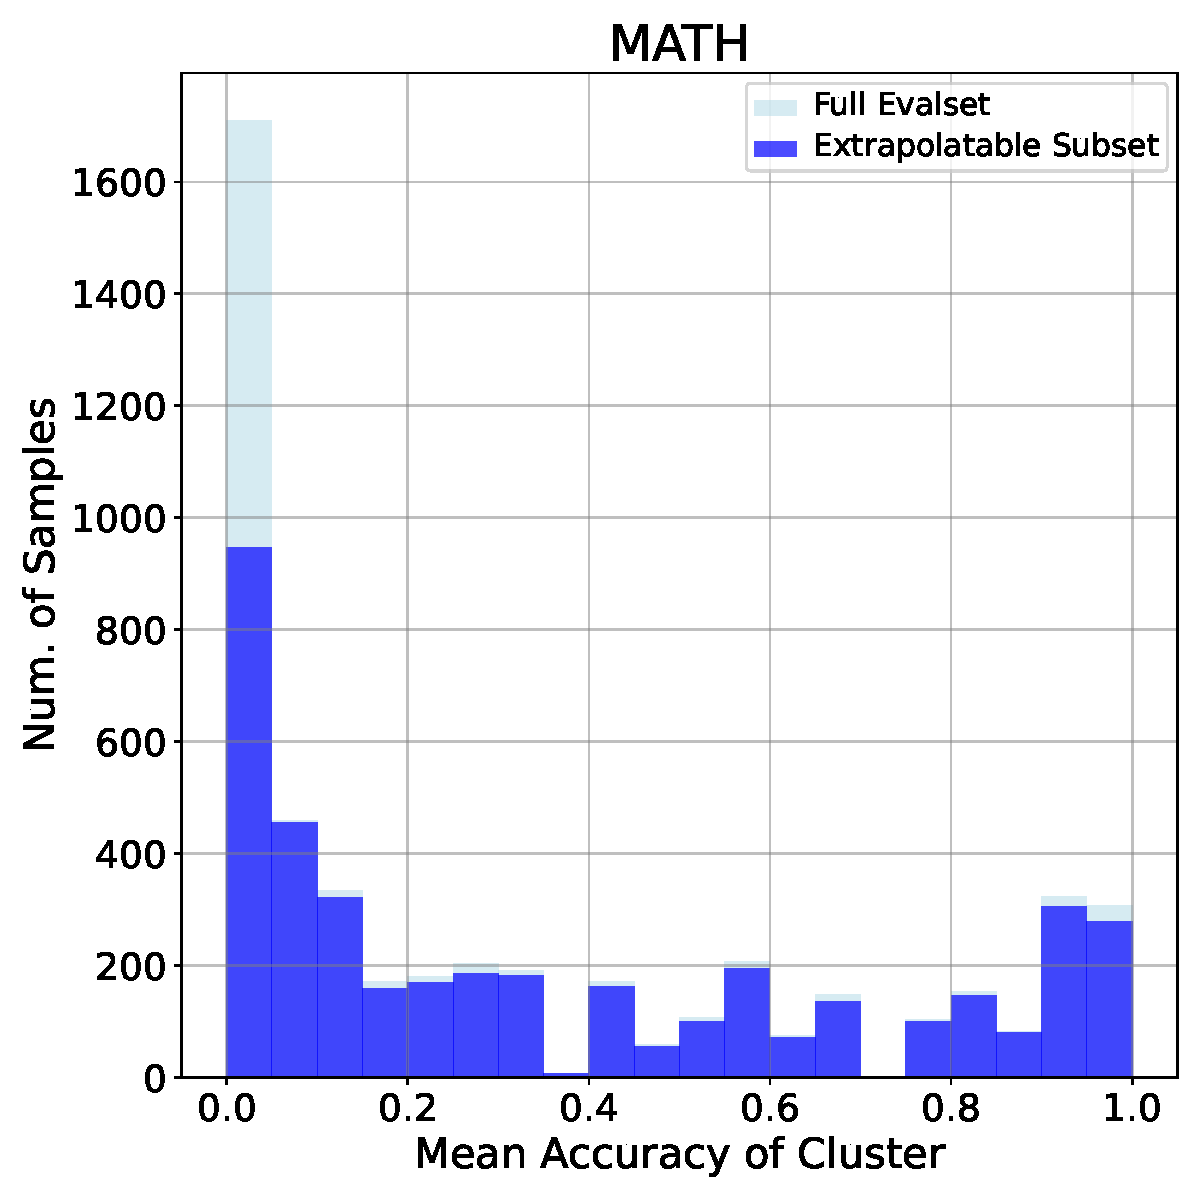
\includegraphics[width=\textwidth]{figures/appendix/difficulty_distributions/math.pdf}
        % \caption*{Title 2}
    \end{minipage}
    \begin{minipage}{0.24\textwidth}
        \centering
        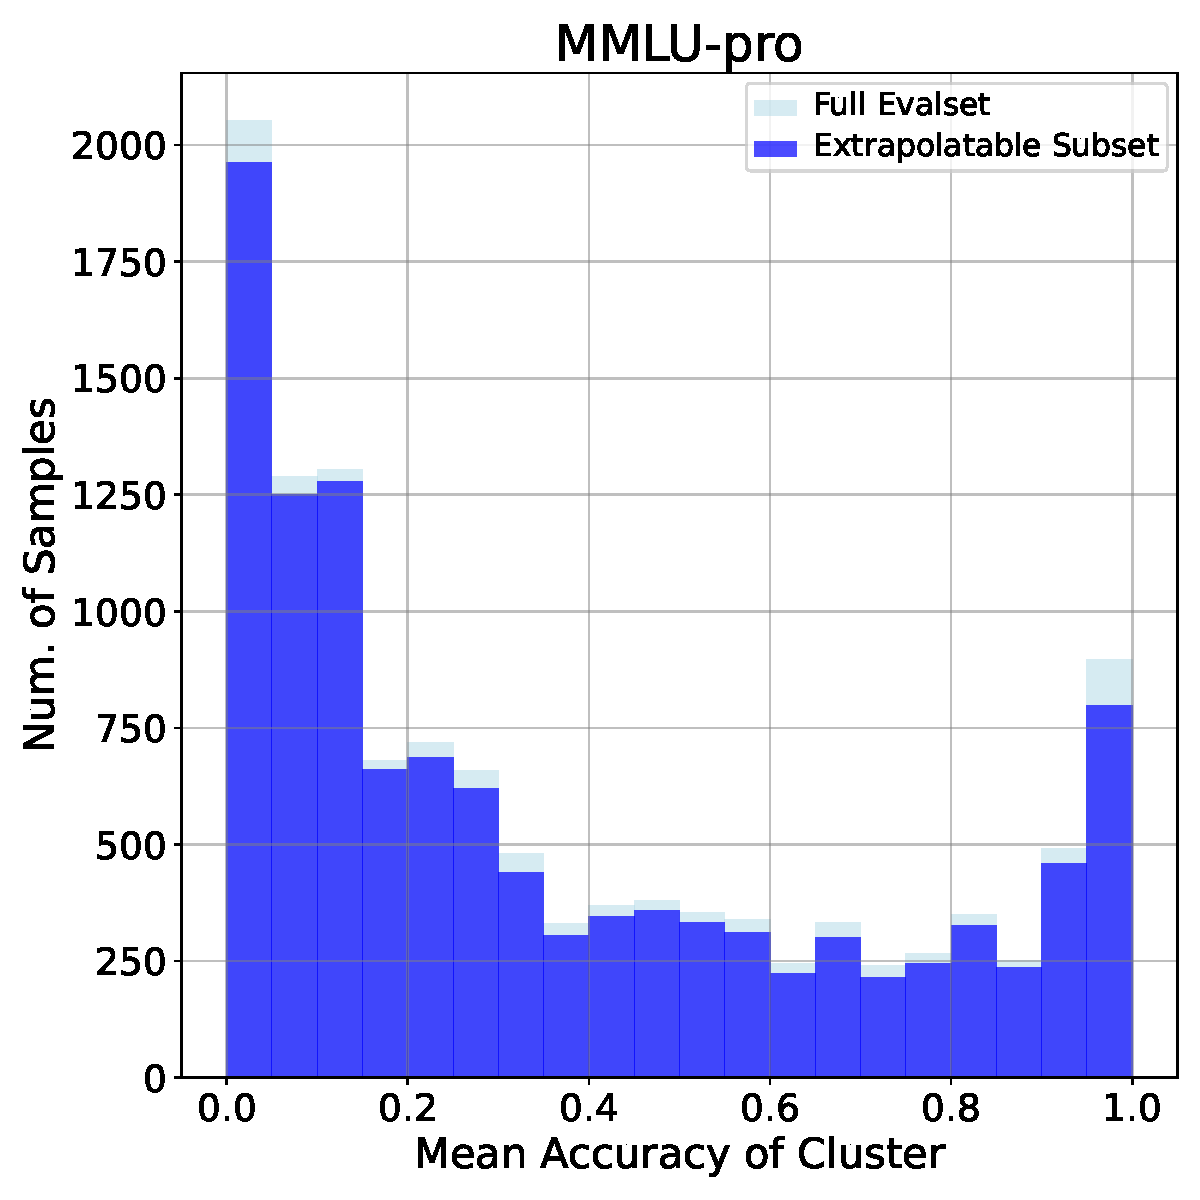
\includegraphics[width=\textwidth]{figures/appendix/difficulty_distributions/mmlu_pro.pdf}
        % \caption*{Title 3}
    \end{minipage}
    \begin{minipage}{0.24\textwidth}
        \centering
        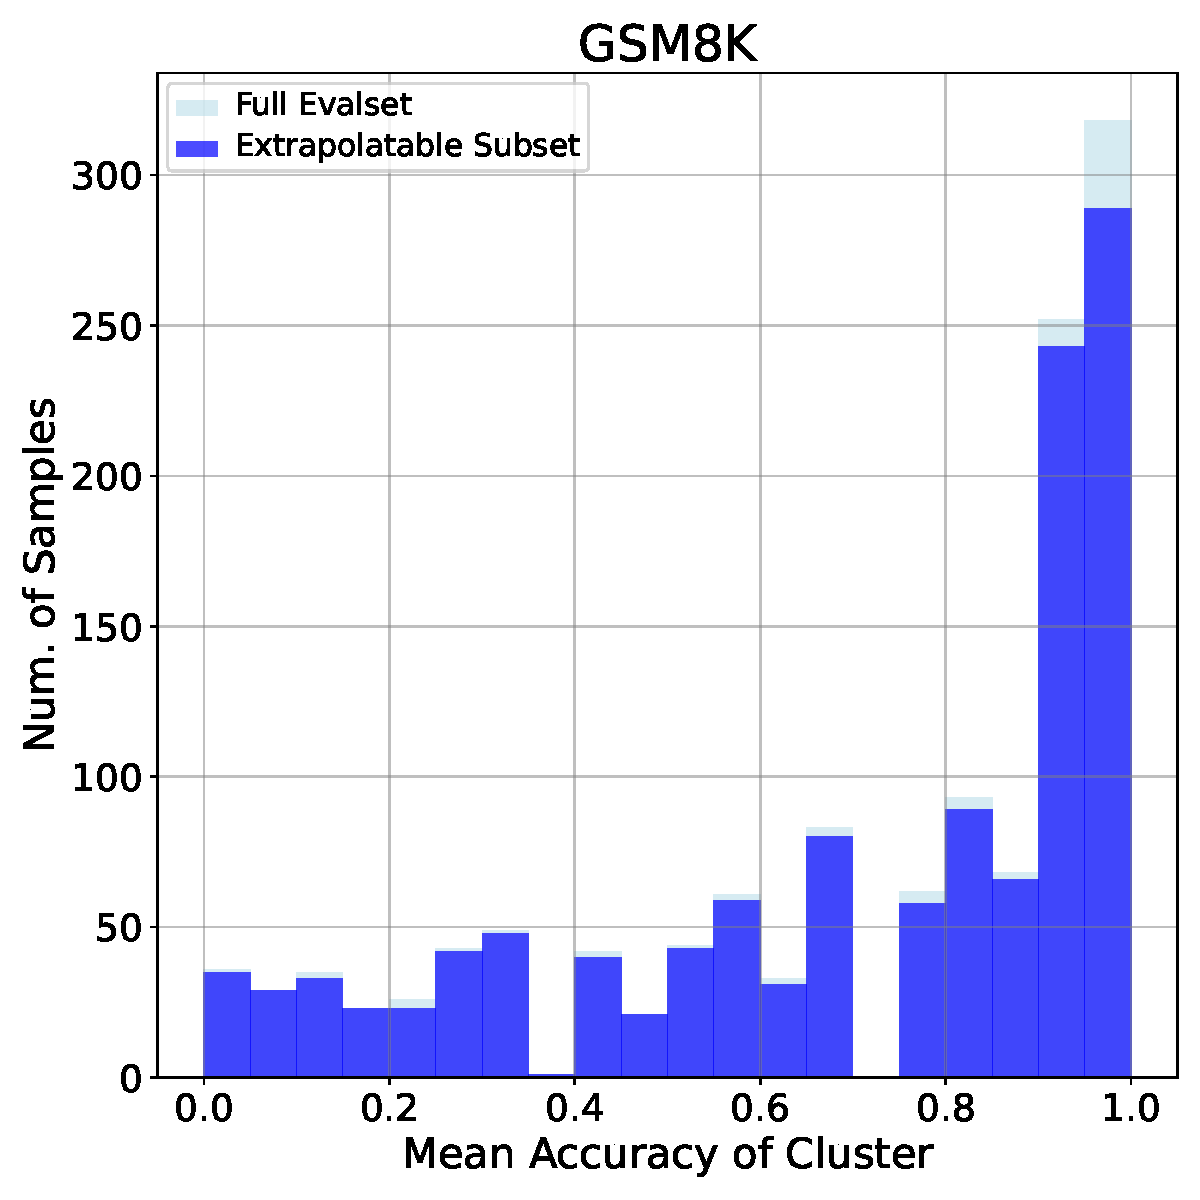
\includegraphics[width=\textwidth]{figures/appendix/difficulty_distributions/gsm8k.pdf}
        % \caption*{Title 4}
    \end{minipage}
    
    \vspace{0.5cm} % Add space between rows
    
    % Second row
    \begin{minipage}{0.24\textwidth}
        \centering
        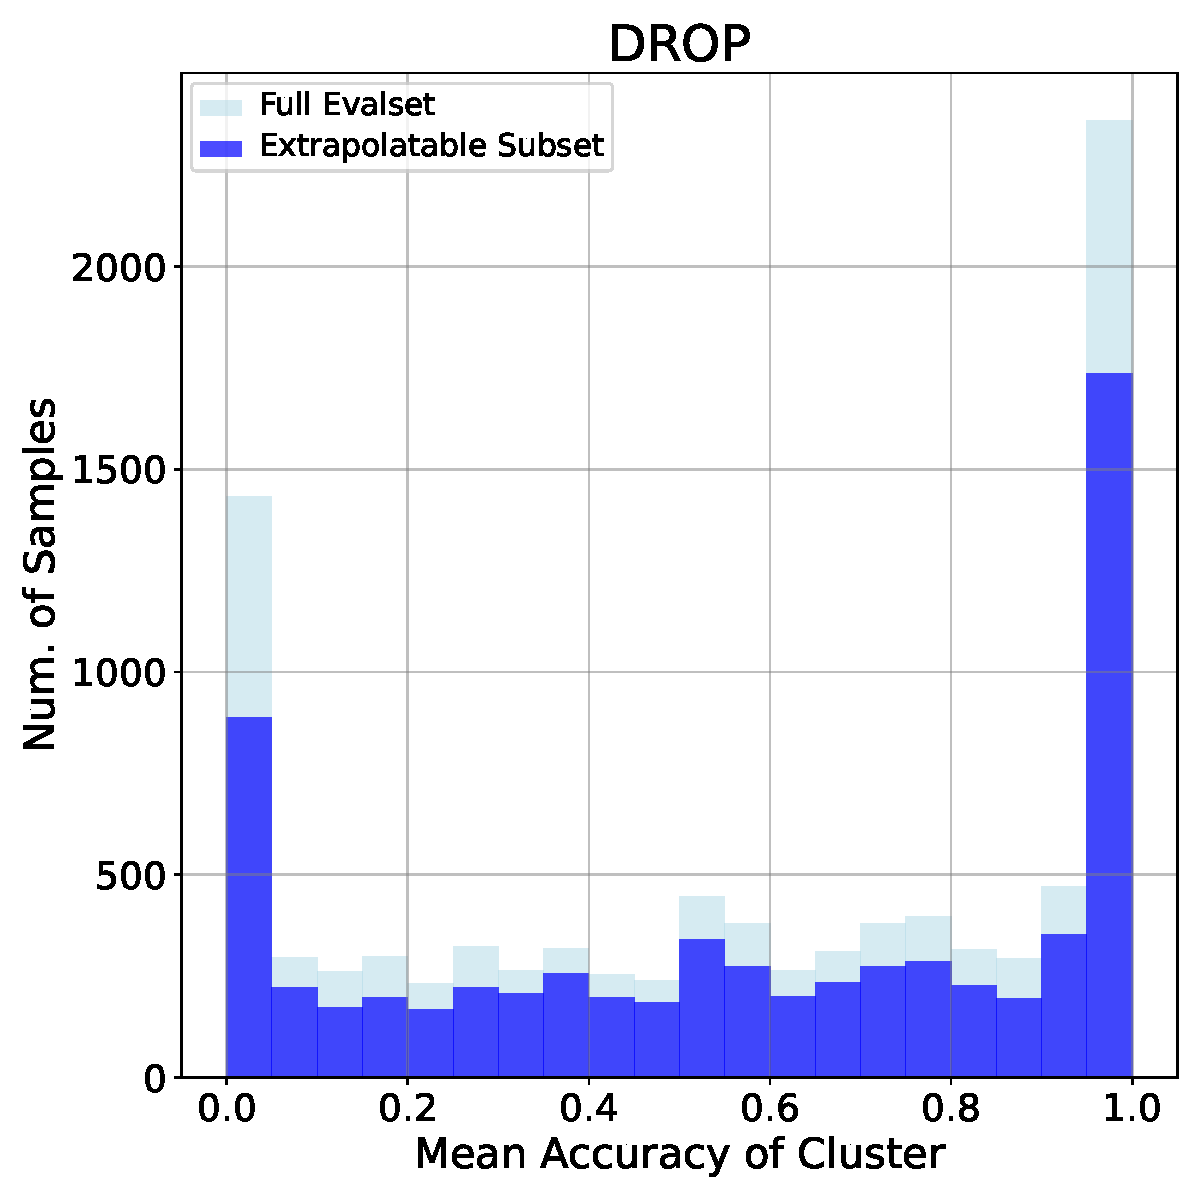
\includegraphics[width=\textwidth]{figures/appendix/difficulty_distributions/drop.pdf}
        % \caption*{Title 5}
    \end{minipage}
    \begin{minipage}{0.24\textwidth}
        \centering
        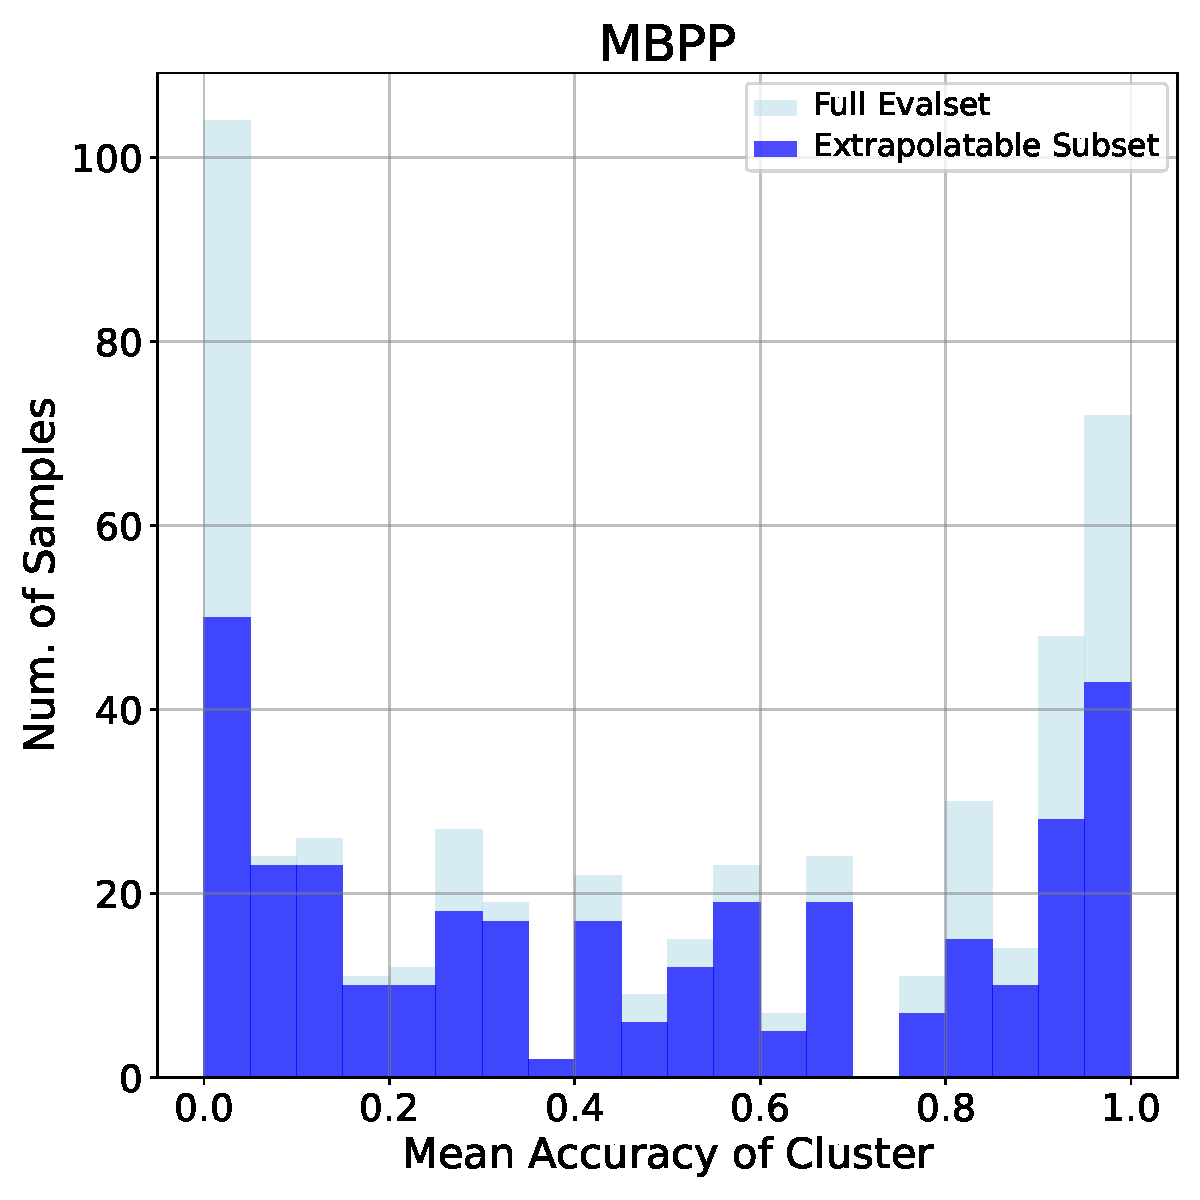
\includegraphics[width=\textwidth]{figures/appendix/difficulty_distributions/mbpp.pdf}
        % \caption*{Title 6}
    \end{minipage}
    \begin{minipage}{0.24\textwidth}
        \centering
        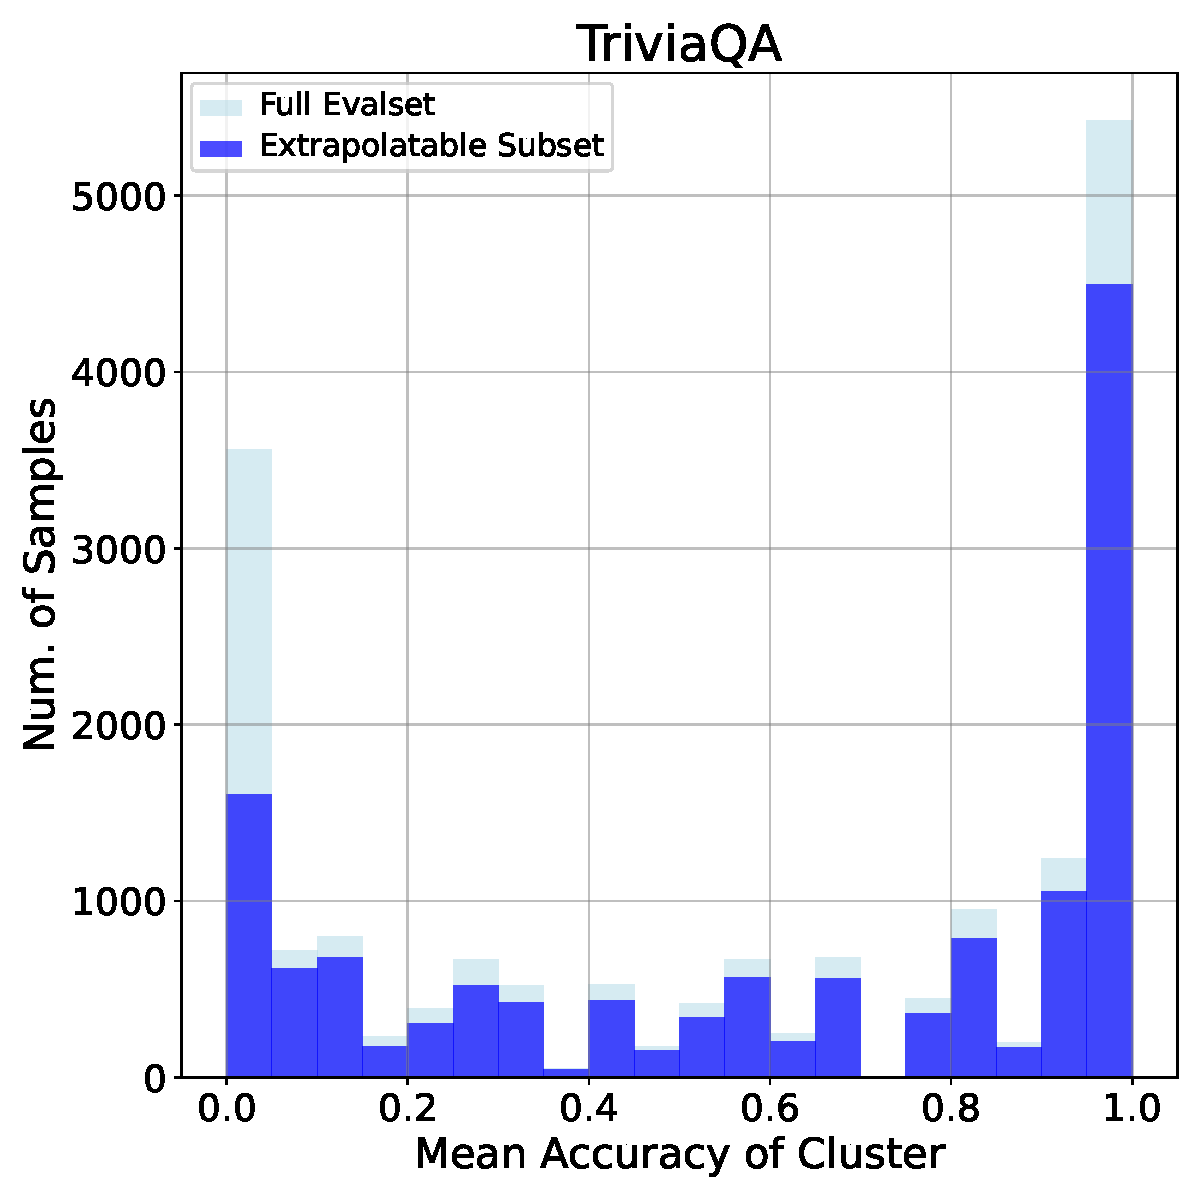
\includegraphics[width=\textwidth]{figures/appendix/difficulty_distributions/triviaqa.pdf}
        % \caption*{Title 7}
    \end{minipage}
    \begin{minipage}{0.24\textwidth}
        \centering
        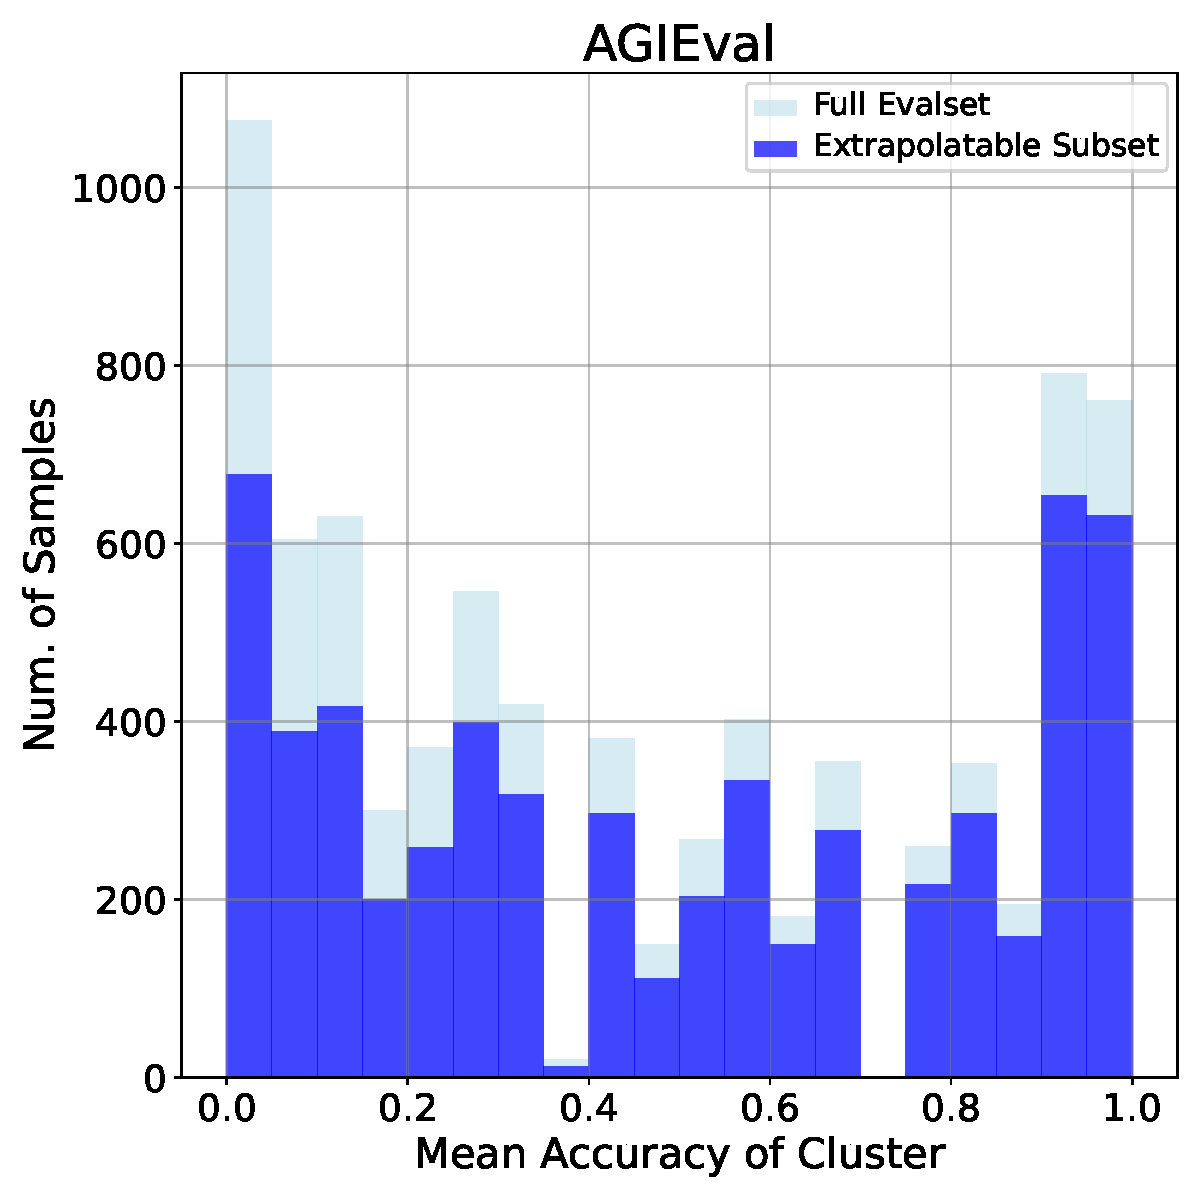
\includegraphics[width=\textwidth]{figures/appendix/difficulty_distributions/agieval.pdf}
        % \caption*{Title 8}
    \end{minipage}
    
    \caption{Difficulty distribution comparison on a 12B model between predictable subset and full evaluation set.}
    \label{fig:diff_dist}
\end{figure}


\renewcommand{\thefigure}{E\arabic{figure}}
\renewcommand{\thetable}{E\arabic{table}}
\renewcommand{\theproposition}{E.\arabic{proposition}}

\section{\anno{Computational Cost}}
\label{append:compute}
\anno{
The extra computational overhead of running COD is not expensive compared to training a series of small models with increasing parameter sizes. The main additional cost comes from performing 100 inference evaluations on the evaluation set for each small model (the cost of clustering algorithm is negligible compared to the inference cost). The computational complexity is $O(TMN)$, where $T$ is the number of evaluation runs, $M$ is the number of tokens for one evaluation, and $N$ is the maximum parameter size of the small models used for prediction. The corresponding token usage is $O(TM)$.

In particular, for an evaluation set requiring $1M$ tokens, a total of $100M$ tokens for small model inference is needed. In our experiments, the training token count for the 12B small model is $1.554T$. Considering that a training token is typically 3 times more costly than an inference token, the additional cost of COD is approximately $\frac{100M}{1.554T * 3} \approx 0.002\%$ of the training cost.
}

% \labubu{Furthermore, the cluster information for an evaluation set characterizes its difficulty distribution (including not only absolute difficulty but also the scaling features of the problems). This information is independent of the specific family of models being evaluated. Therefore, these clusters can be reused when estimating the capabilities of LLMs with new architectures, parameter counts, or training data.}

\section{Limitations}
\label{sec:limiations}

% \noindent\textbf{Influence of model structure.} Mixture-of-Experts (MoE) models excel in training and inference cost, and are widely used in production. In this work, we reveal the performance scaling on dense transformers, while prediction on MoE models is still underexplored.
% % 不过我们认为所提方法不会收到模型结构影响很多，如果我们把完整Pipeline应用在MoE模型上，我们同样预期能获得相似效果。
% However, we believe that the proposed method is not significantly affected by the model architecture. We expect similar results for MoE models.
% 我们只研究了恒定学习率的预训练能力预估，没有覆盖到退火阶段对指标的影响。该阶段通常采用更高质量的数据，可以快速提升模型能力，也因此Performance Prediction具有更大挑战。


\noindent\textbf{\camera{Compromised robustness due to excessive hyperparameter.}}
\camera{The complete pipeline of our proposed COD method incorporates several hyperparameters designed to constrain and refine the outcomes of various stages. These include the minimum intra-cluster sample size $K$, the adaptive bandwidth hyperparameter $Q$, and the maximum intra-cluster distance threshold $U$ for the clustering phase; parameters $a, b,$ and $c$ for filtering extrapolatable subsets during curve fitting; and the RMSE threshold $T$ utilized during the mapping process.

Regarding the clustering-related hyperparameters, they can be omitted if pre-computed cluster assignments are reused; otherwise, we provide empirically validated default values as reliable priors. For the remaining hyperparameters, we present comprehensive ablation studies in the paper, demonstrating that the final predictive performance is robust and relatively insensitive to these settings. Despite these mitigations, the reliance on a multi-parameter configuration may pose challenges to the COD method’s ease of deployment when generalizing to novel prediction scenarios.}
% 我们提出的COD方法的完整pipeline中存在较多的超参数用于约束各个阶段的效果，包括聚类时的最小类内样本数K、自适应带宽超参数Q、类内最大距离值，拟合曲线时用于筛选可外推子集的a、b、c，以及mapping时RMSE的阈值B。对于前三个聚类相关的超参数，如果复用已有聚类结果则可以省略；如果需要重新进行聚类，我们也提供了先验较为合理的参考值。对于后四个超参数，我们在文中给出了充足的超参消融实验验证了鲁棒性，证明最终预测效果对这些超参不敏感。尽管如此，较多的超参数还是使得COD方法在迁移到新预测场景下时的鲁棒性受到挑战。

\noindent\textbf{Category of evaluation sets.}
% 我们提出的Clustering-on-Difficulty Method对测试集题目数量有一点要求，过少的题目导致类簇指标不稳定从而无法有效预估。不过从测试集设计的角度看，一个具有良好预估性质的评估集可以更有效的通过小模型实验结果推广到大模型，对于模型迭代具有更好的指导意义。
%
%此外，针对Multi-choice类型题目，仅需要保证预测出正确选项概率大于其余选项，此时指标与模型真实的Passrate存在差异。考虑到更多的评估集采用Chain-of-Thoughts模式，我们没有覆盖近输出选项的选择题任务。
The proposed Clustering-on-Difficulty method requires a sufficient number of test cases, as too few samples can lead to unstable cluster metrics and ineffective estimation. From an evaluation set design perspective, an evaluation set with good predictive properties enables more effective generalization from small-scale to large-scale models, thus providing better guidance for model iteration.

\revise{Furthermore, we have not included multiple-choice tasks that require comparing the logits of correct options to calculate scores. These tasks creating a discrepancy between the answer loss and the model's true passrate, which violates the assumptions of the proposed Scaling Law for downstream task performance.}

\noindent\textbf{\camera{The prediction accuracy for smaller models is unsatisfactory.}}
\camera{Since our proposed COD (Clustering on Difficulty) method involves modeling the scaling of sample difficulty within the evaluation set, the clustering process requires a certain scale of models to participate in pass rate evaluation. This ensures an accurate estimation of sample difficulty. However, when predicting the performance of relatively smaller target models (e.g., around 10B parameters), the proxy models used for clustering and fitting are typically limited to even smaller scales (e.g., 2B). In such scenarios, a significant portion of samples may exhibit non-emergent or nascent emergent behaviors, making it challenging to accurately model difficulty features that scale with compute. Under these specific constraints, methods that perform sample-wise extrapolation—such as PassUntil~\citep{hu2023predicting}—tend to yield more robust predictive performance. Nonetheless, the primary utility of metric prediction lies in forecasting the downstream performance of significantly larger models. From this perspective, our COD method maintains broad applicability and significant value in mainstream scaling law research.}
% 由于我们提出的COD方法涉及对评估集样本难度scaling的建模，因此在聚类时需要一定规模的模型参与passrate评估，以保障对样本难度的准确估计。在预测smaller model（如10B左右）时，用于聚类、拟合的小模型最大可能也只有2B左右，此时会出现大量的未涌现或刚涌现的样本，无法准确建模随算力scaling的难度特征。在这种场景下，直接利用 passrate 指标 sample-wise外推再聚合的预测效果会更理想，如PassUntil方法。不过从另一个角度说，metric prediction方法更重要的应用还是预测更大的模型的下游指标，因此我们提出的COD方法依然有广泛的使用价值。

\noindent\textbf{Chain-of-thought performance prediction}.
% 我们提出的Scaling Law for Downstream Tasks~\cref{proof:task_scaling_law}假设了测试集评价模型直接给出答案的能力。但实际上越来越多的评测会允许模型进行思考后给出答案。Inference time scaling更进一步表明在数学、推理、代码等任务上，通过训练模型通过更长推理计算来完成任务可以大幅提升下游任务效果。
% 在推理过程或答案不唯一的情况下，模型在一个Task的Answer Loss与其Passrate不一定具有$p_\mathrm{ans}=\exp(-\mathrm{loss}_\mathrm{ans})$的关系。虽然我们的方案在该情况下保持其预估效果，但理论解释是不充分的。因此，我们把根据Chain-of-thought特性改进预估方法与扩充理论依据作为未来工作。
\cref{main:proof:task_scaling_law} assumes that evaluation sets directly assess models' ability to provide answers. However, increasingly more evaluations allow models to think before providing answers. Recent works on inference time scaling~\citep{snell2024scaling, bansal2024smaller} further demonstrate that for tasks involving mathematics, reasoning, and coding, training models to complete tasks through longer inference computation can significantly improve downstream task performance. In cases where the reasoning process or answers are not unique, the relationship between a model's answer loss and passrate on a task may not necessarily follow the exponential relationship between the answer loss and the sample passrate. \camera{Although our COD framework still achieves reasonable prediction performance in such scenarios, its theoretical foundation lacks sufficient explanation for the performance scaling of chain-of-thought based tasks.} Therefore, we consider improving prediction methods based on chain-of-thought characteristics and expanding theoretical foundations as future work.

% \noindent\textbf{\labubu{Complex Procedure.}}
% \labubu{Compared with current mainstream prediction methods (Loss-intermediate or End-to-end methods), the proposed COD requires more preparatory efforts and involves a more complex prediction process, which poses substantial challenges to both the reproduction of this method and its practical application in the prediction of LLMs. In future work, we will attempt to simplify the preparatory efforts and prediction process, or release a robust set of clustering labels for open-source evaluation datasets, thereby reducing the overhead for the academic community to reproduce or apply this method.}

% \section{Use of LLMs}
% \label{sec:llmuse}
% We utilized language models at the writing level, including checking for grammatical errors in the article, modifying expressions, and translating non-English information. The language models had no impact on the article's innovative contributions, experiments, or analytical perspectives.
